% Template:     Template Tesis LaTeX
% Documento:    Archivo principal
% Versión:      1.1.7 (02/10/2019)
% Codificación: UTF-8
%
% Autor: Pablo Pizarro R. @ppizarror
%        Facultad de Ciencias Físicas y Matemáticas
%        Universidad de Chile
%        pablo.pizarro@ing.uchile.cl, ppizarror.com
%
% Sitio web:    [https://latex.ppizarror.com/tesis]
% Licencia MIT: [https://opensource.org/licenses/MIT]
% CREACIÓN DEL DOCUMENTO
\documentclass[letterpaper,12pt,oneside]{book} % Libro, tamaño carta
\usepackage[utf8]{inputenc} % Codificación UTF-8

\bibliographystyle{unsrtnat}
% INFORMACIÓN DEL DOCUMENTO
\def\titulotesis {Modelamiento y seguimiento de tópicos para detección de modus operandi en robo de vehículos}
\def\titulogrado {
	Tesis para optar al grado de magíster en gestión de operaciones
	\bigbreak\vspace{0.3cm}
	Memoria para optar al título de ingeniero civil industrial
}

\def\nombreuniversidad {Universidad de Chile}
\def\nombrefacultad {Facultad de Ciencias Físicas y Matemáticas}
\def\departamentouniversidad {Departamento de Ingeniería Industrial}
\def\imagendepartamento {img/dptos/uchile2.pdf}
\def\imagendepartamentoescala {0.7}
\def\localizacionuniversidad {Santiago, Chile}

% INTEGRANTES, PROFESORES Y FECHAS
\def\autortesis {DIEGO GARRIDO}
\def\fechatesis {\the\year}

\def\tablacomision {
\begin{tabular}{c}
	\vspace{1.5cm} \\
	\MakeUppercase{\textbf{\autortesis}} \\
	\vspace{1.0cm} \\
	PROFESOR GUÍA: \\
	RICHARD WEBER \\
	\vspace{0.5cm} \\
	MIEMBROS DE LA COMISIÓN: \\
	GIORGIOGIULIO PARRA\\
	%PROFESOR 3 \\
	\vspace{0.5cm} \\
	\MakeUppercase{\localizacionuniversidad} \\
	\MakeUppercase{\fechatesis}
\end{tabular}}{
}
\def\tablaresumen {
\begin{tabular}{l}
	RESUMEN DE LA MEMORIA PARA OPTAR \\
	AL TÍTULO DE MAGÍSTER EN CIENCIAS \\
	DE LA INGENIERÍA \\
	POR: \MakeUppercase{\textbf{\autortesis}} \\
	FECHA: \MakeUppercase{\fechatesis} \\
	PROF. GUÍA: RICHARD WEBER
\end{tabular}}{
}

% CONFIGURACIONES
\input{lib/config}

% IMPORTACIÓN DE LIBRERÍAS
\input{lib/env/imports}
\graphicspath{img/} 

% IMPORTACIÓN DE FUNCIONES Y ENTORNOS
\input{lib/cmd/all}

% IMPORTACIÓN DE ESTILOS
\input{lib/style/all}

% CONFIGURACIÓN INICIAL DEL DOCUMENTO
\input{lib/cfg/init}

% TODONOTES
\usepackage{todonotes}

% INICIO DE LAS PÁGINAS
\begin{document}

% PORTADA
\input{lib/page/portrait} % Se puede borrar

% CONFIGURACIÓN DE PÁGINA Y ENCABEZADOS
\input{lib/cfg/page}

% DEDICATORIA
\begin{dedicatoria}
	\todo[inline]{TODO}
\end{dedicatoria}

% AGRADECIMIENTOS
\begin{agradecimientos}
    \todosec[inline]{TODO}
\end{agradecimientos}

% TABLA DE CONTENIDOS - ÍNDICE
\input{lib/page/index}

% RESUMEN O ABSTRACT
\begin{resumen}
	\todo[inline]{Actualizar tras terminar la conclusión}
    En este trabajo se describe una metodología para el descubrimiento de tópicos en el tiempo. La metodología propuesta está basada en (i) discretización del corpus en épocas, (ii) descubrimiento de tópicos en cada época mediante Hierarchical Dirichlet Process (HDP), (iii) la construcción de un grafo de similitud entre tópicos de épocas adyacentes, el cual permite modelar cambios entre los tópicos como: nacimiento, muerte, evolución, división y fusión. En contraste a trabajos anteriores, la metodología propuesta utiliza Word Mover's Distance (WMD) como medida de similitud entre tópicos, medida que destaca por ser robusta a tópicos que no poseen un vocabulario común, debido a que trabaja con sus \textit{word embeddings}. Se reportan resultados experimentales tanto cuantitativos como cualitativos en el fenómeno de robo de vehículos en Chile, usando como corpus los relatos de víctimas de robo de vehículo entre los años 2011-2016 provistos por la Asociación de Aseguradores de Chile (AACH). El algoritmo propuesto logra capturar bien los tópicos latentes del corpus, descubriendo delitos tales como \quotes{portonazo}, apropiación indebida y robo con violencia.
\end{resumen}

% CONFIGURACIONES FINALES
\input{lib/cfg/final}
\hypersetup{
    citecolor=Blue
}

% CONFIGURACIÓN TODONOTES 
% \reversemarginpar
% \setlength{\marginparwidth}{2.0cm}
% ======================= INICIO DEL DOCUMENTO =======================
\listoftodos
\chapter{Introducción}
\label{ch:introduction}
Grandes volumenes de datos digitales son almacenados día a día, en forma de noticias, blogs, páginas web, artículos científicos, libros, imágenes, sonido, video, redes sociales, etc. Volviéndose clave contar con herramientas computacionales que ayuden a organizar, buscar y entender grandes colecciones de datos.\\

Al buscar y explorar documentos en base a sus temas, se podría enfocar la búsqueda en temas específicos o más amplios, se podría observar como estos temas cambian en el tiempo o como se relacionan unos a otros. En vez de buscar documentos únicamente a través de palabras claves, se podría primero hallar temas de interés, y luego examinar los documentos relacionados a ese tema. Por ejemplo, se podría descubrir nuevas tendencias de investigación, analizar la evolución de la contigencia social, estudiar la efectividad de campañas publicitarias en base a la opinión de los consumidores, organizar y recomendar contenido en un blog, etc.\\

El objetivo del trabajo de tesis es desarrollar una metodología que permita descubrir tópicos en el tiempo, siendo capaz de modelar cambios tales como: nacimiento, muerte, evolución, división y fusión. Adicionalmente, debe ser robusta a cambios en el vocabulario en el tiempo, permitiendo comparar tópicos de épocas adyacentes a pesar que de no tener un vocabulario común.

\section{Metodología Propuesta}
Los modelos de tópicos probabilísticos ayudan a descubrir los temas latentes (\textit{clusters}) en una colección de documentos, como estos temas están conectados unos a otros y cómo cambian en el tiempo. Permiten resumir un gran colección de documentos a través de sus temas y organizarlos entorno a estos. Estos tratan a un tópico como una distribución de probabilidad discreta sobre el vocabulario de un corpus. Una práctica habitual es interpretar un tópico a partir de sus $N$ palabras más probables. Por ejemplo, para $N=5$ las palabras más probables de un tópico son: \quotes{llaves}, \quotes{domicilio}, \quotes{individuos}, \quotes{casa} y \quotes{porton}, por lo que una etiqueta valida para este tópico podría ser \quotes{portonazo}.\\ 

En esta tesis se propone una metodología para el descubrimiento de tópicos en el tiempo. Esta metodología consiste en la discretización del corpus en épocas, el descubrimiento de tópicos en cada época mediante Hierarchical Dirichlet Process (HDP), la construcción de un grafo de similitud entre tópicos de épocas adyacentes, el cual permite modelar cambios entre los tópicos como: nacimiento, muerte, evolución, división y fusión. En contraste a trabajos anteriores, la metodología propuesta utiliza Word Mover's Distance (WMD) como medida de similitud entre tópicos. Esta medida destaca por su robustez ante tópicos que no poseen un vocabulario común, debido a que trabaja sobre el espacio de los \textit{word embeddings}.\\

\section{Caso de estudio}

Se escoge el problema del robo de vehículos o accesorios de vehículos como caso de estudio, debido a que es un problema que afecta a toda la sociedad en Chile y en el mundo, problema que se ha vuelto más relevante el último tiempo debido al crecimiento en el robo de vehículo motorizado y accesorios (ver Figura \ref{fig:antecedente}).\\ 

\begin{figure}
    \includegraphics[width=1\textwidth]{ch1/robberies.eps} 
    \caption{Cantidad de robos de vehículos y accesorios anuales en Chile entre los años 2006-2016. Fuente: Informe anual de Carabineros, 2006-2016, INE.} 
    \label{fig:antecedente}
\end{figure}

Este fenómeno trae consigo un montón de costos para la sociedad, como incremento en la percepción de la seguridad, aumentos en la prima de los seguros de los asegurados, aumento en los costos de las aseguradoras \footnote{Considerando que el costo promedio incurrido en un auto asegurado robado y no recuperado es de \$ 5,000,000 de pesos, la pérdida total considerando solo los vehículos no recuperados para el año 2015 es de unos \$15,720 millones de pesos.} y el incremento de otros tipos de delitos. \footnote{El destino de los vehículos robados es variado, se usan los autos para perpetrar otros delitos y huir, venderlos por piezas en talleres clandestinos o blanquear sus documentos para pasarlos por la frontera y venderlos o cambiarlos por otros bienes en el extranjero.}\\

El corpus utilizado correspode a una colección de 49,015 relatos de víctimas de robo de vehículo, entre los años 2011-2016, provistos por la Asociación de Aseguradores de Chile (AACH). Cabe destacar que se estima que un tercio del parque automotriz se encuentra asegurado\footnote{\href{http://www.economiaynegocios.cl/noticias/noticias.asp?id=185224}{http://www.economiaynegocios.cl/noticias/noticias.asp?id=185224}}, por lo que se trabaja con una muestra del parque automotriz.\\

En el contexto de robo de vehículos, los tópicos pueden interpretarse como los \quotes{modus operandi} que utilizan los delicuentes para robar un vehículo. Así, la metodología propuesta permite descubrir los \textit{modus operandi} ocultos en los relatos de las víctimas y caracterizarlos a partir de las palabras, como también ver su evolución a través del tiempo, siendo capaz de detectar cuando nacen y mueren, y como cambian en el tiempo.\\

\section{Revisión del estado del arte}

El problema enunciado consiste en una tarea de \textit{clustering}, debido a que no se cuenta con una etiqueta del tema al que corresponde cada documento, siendo el propósito del trabajo descubrirla. El modelamiento de tópicos es uno de los enfoques más prometores de \textit{clustering} aplicado a texto, siendo su objetivo descubrir los temas (\textit{clusters}) ocultos presentes en el corpus, permitiendo resumir, organizar y explorar grandes colecciones de datos.\\

Algunas de las técnicas de modelamiento de tópicos están basadas en factorización matricial como LSI (Latent Semantic Indexing) \citep{dumais2004latent} o NMF (Non-negative Matrix Factorization) \citep{xu2003document}, pero este trabajo está basado en modelos probabilísticos generativos, como LDA (Latent Dirichlet Allocation) \citep{blei2003latent} o HDP (Hierarchical Dirichlet Process) \citep{teh2005sharing}. Ambos enfoques tienen sus pros y contras, en este trabajo se escoge el enfoque probabilístico ya que es capaz de expresar incertidumbre en la asignación de un tópico a un documento y en la asignación de palabras a los tópicos, además, este enfoque suele aprender tópicos más descriptivos \citep{stevens2012exploring}.\\

En el modelamiento de tópicos se pueden presentar los siguientes dinamismos:
\begin{enumerate}
    \item \textbf{Evolución de los tópicos}: la evolución de los tópicos se refleja en el cambio en la distribución sobre las palabras. Por ejemplo, el \quotes{portonazo} en un determinado momento se comete en grupos de 2-3 personas con arma blanca, luego evoluciona de arma blanca a arma de fuego y lo perpetran jóvenes menores de edad.
    \item \textbf{Dinámismo en la mezcla de tópicos}: esto permite capturar la popularidad de los tópicos en el tiempo.
    \item \textbf{Nacimiento, muerte, fusión y división de tópicos}: En el contexto de robos es natural que en el tiempo aparezcan nuevos \textit{modus operandi} como también que desaparezcan aquellos que ya no parecen tan atractivos.
\end{enumerate}

En el modelamiento de tópicos estático destaca LDA y HDP. La diferencia principal es que LDA necesita de antemano fijar el número de tópicos a descubrir y HDP lo infiere a partir del corpus.\\

Dentro de los primeros modelos de tópicos dinámicos exitosos está Dynamic Topic Modelling (DTM) junto Topic Over Time (TOC)\citep{wang2006topics}. Estos modelos mantienen el número de tópicos fijo en el tiempo, por lo que si aparece un nuevo tópico este quedará clasificado dentro de un tópico preexistente desde el comienzo, por lo que solo es capaz de capturar el punto 1 y 2.\\

En \citep{ahmed2012timeline} se propone Dynamic Hierarchical Dirichlet Process (DHDP), modelo que no mantiene el número de tópicos fijo en el tiempo, sino que lo infiere a partir del corpus. Sin embargo, este modelo no es capaz de capturar fusión y división de tópicos. Además, a diferencia de los otros modelos de tópicos mencionados, DHDP no es una tecnología ampliamente usada y no cuenta con una implementación disponible, por lo que se desconoce su desempeño en otras fuentes de información.\\

En \citep{wilson2011tracking} y \citep{beykikhoshk2018discovering} se propone una metodología que permite capturar los dinámismos mencionados utilizando LDA y HDP respectivamente. Estas consisten en dividir el corpus en épocas, entrenar de forma independiente un modelo de tópico en cada época, para finalmente unir los resultados obtenidos. En este trabajo se utilizan técnicas de modelado dinámico de tópicos bajo este enfoque, usando HDP para el descubirmiento de tópicos en cada época.

\section{Estructura de la tesis}
En el capítulo \ref{ch:theorethical_framework} se describen los fundamentos teóricos en los que se basa la metodología propuesta la cual es descrita en el capítulo \ref{ch:methodology}. Luego, en el capítulo \ref{ch:case_study} se presenta un análisis cuantitativo y cualitativo de la metodología propuesta en el fenómeno de robo de vehículos. Finalmente, en el capítulo \ref{ch:conclusion} se presentan las conclusiones y futuras lineas de investigación.


\chapter{Marco teórico}
\label{ch:theorethical_framework}
En este capítulo se describen los conceptos fundamentales para comprender la metodología propuesta en el capitulo \ref{ch:methodology}. El capítulo es estructurado como sigue. En la sección \ref{sec:mixture_models} se introduce a nivel general los modelos de \textit{clustering} probabiĺísticos conocidos como \textit{mixture models}. En la sección \ref{sec:topic_models} se describen los modelos de tópicos estáticos LDA y HDP. Finalmente, en la sección \ref{sec:topic_evolution} se explica una metodología que modela la evolución de los tópicos en el tiempo. 

\section{Mixture Models}
\label{sec:mixture_models}

Uno de los supuestos básicos en \textit{clustering} es asumir que cada observación $x_{i}$ pertenece a un solo \textit{cluster} $k$. La asignación a un \textit{cluster} se puede expresar como una variable aleatoria $z_{i}$, donde $z_{i}=k$ significa que $x_{i}$ pertenece al \textit{cluster} $k$. La variable $z_{i}$ no es observada en los datos y se considera una variable oculta. Cada \textit{cluster} posee un parámetro $\phi_{k}$ que codifica su información. La distribución que caracteriza a un solo \textit{cluster} $k$ condicionando en $z_{i}$ es

\begin{align}
    p(x_{i}|z_{i}=k, \phi) = p(x_{i}|\phi_{k})\\
\end{align}

Además, la probabilidad de que una nueva observación pertenezca al \textit{cluster} $k$ se define como 

\begin{align}
    p(z_{i}=k|\pi) = \pi_{k}
\end{align}

Con $\sum_{k}\pi_{k} = 1$, ya que $\pi_{k}$ son probabilidades de eventos mutuamente excluyentes. La distribución de $x_{i}$ es de la forma

\begin{align}
  p(x_{i}) = \sum_{k}p(z_{i}=k|\pi)p(x_{i}|z_{i}=k, \phi) = \sum_{k}\pi_{k}p(x_{i}|\phi_{k})
\end{align}

La distribución $p(x_{i}|\phi_{k})$ se denota $x_{i} \sim F(\phi_{z_{i}})$, donde $F$ es la distribución asociada a las observaciones. \\

Una representación equivalente se obtiene al considerar el parámetro $\phi_{z_{i}}$ usado para generar la observación $x_{i}$ proviene de una distribucion discreta $G$, la cual tiene la forma

\begin{align}
    G(\phi) & = \sum_{k} \pi_{k}\delta_{\phi_{k}}(\phi)
\end{align}

En otras palabras, $G$ es una mezcla de funciones delta, donde la probabilidad de que $\phi$ sea igual a $\phi_{k}$ es $\pi_{k}$. Luego, un \textit{mixture model} se puede  representar como a continuación

\begin{align}
\phi_{z_{i}} & \sim G\\
x_{i} & \sim  F(\phi_{z_{i}})
\end{align}

Un \textbf{Bayesian mixture model} es un \textit{mixture model} con una medida aleatoria para las mezclas. En las secciones \ref{sec:dirichlet}. y \ref{sec:dp} se describen dos \textit{priors} ampliamente usados para construir \textit{bayesian mixture model}: la distribución Dirichlet que permite construir un \textbf{finite mixture model}, donde el número de átomos o \textit{clusters} a descubrir es finito, denotado por $K$ y un \textit{prior} no paramétrico denominado Dirichlet Process (DP), el cual permite construir un \textbf{infinite mixture model}, donde el número de \textit{clusters} no está acotado. 

\subsection{Distribución Dirichlet}
\label{sec:dirichlet}

La distribución Dirichlet \citep{minka2000estimating} es una generalización multivariada de la distribución beta, la cual tiene soporte sobre un \textbf{simplex}, definido por:
\begin{equation}
    S_{K} = \big\{x: 0\leq x_{k} \leq 1, \sum_{k=1}^{K}x_{k}=1\big\}
\end{equation}
Luego, su función de densidad de probabilidad (pdf):

\begin{equation}
    Dir(x|\alpha)=\frac{1}{B(\alpha)}\prod_{k=1}^{K}x_{k}^{\alpha_{k}-1}\mathbb{I}(x\in S_{K})
\end{equation}

, donde $B(\alpha) = B(\alpha_{1}, \ldots, \alpha_{K})$ es la generalización de la función beta a $K$ variables:

\begin{align}
    B(\alpha) \triangleq \frac{\prod_{k=1}^{K}\Gamma(\alpha_{k})}{\Gamma(\alpha_{0})}
\end{align}

, donde $\alpha_{0} \triangleq \sum_{k=1}^{K}\alpha_{k}$.\\

En la Figura \ref{img:dirichlet_distribution} se observa el efecto de los parámetros en la distribución Dirichlet con $K=3$. El parámetro $\alpha_{k}$ controla la \textit{sparsity}, mientras más se acerca a 0 los vectores generados tienen más átomos nulos y se concentra la masa en unas pocas coordenadas, mientras más grande $\alpha_{k}$ la masa más se concentra en el centro (1/3, 1/3, 1/3). Cuando $\alpha_{k}=1$ se tiene una distribución uniforme en el dominio $S_{K}$. Por otro lado, cuando $\alpha$ no es simétrico la masa se concentra proporcionalmente en las coordenadas con $\alpha_{k}$ mayor.\\

\begin{figure}
    \centering
    \includegraphics[width=\textwidth]{ch2/dirichlet_simplex.eps}
    \caption{Densidad de la distribución Dirichlet con $K=3$. Define una distribución sobre un \textit{simplex}, el cual puede ser representado por una superficie triangular.}
    \label{img:dirichlet_distribution}
\end{figure}

En general se asume simetría en los parámetros de la distribución Dirichlet de la forma $\alpha_{k}=\frac{\alpha}{K}$, de esta manera $\alpha$ funciona como parámetro de concentración. En la Figura \ref{img:dirichlet_samples} se oberva una realización de una distribución Dirichlet con $\alpha \in \{0.1, 1, 10\}$ y $K\in\{2, 10, 100\}$. En esta figura podemos observar que a mayor $\alpha$ los compenentes del vector $x$ más similares se vuelven, esto es más notorio a mayor dimencionalidad debido a que existen más dimensiones a las que distribuir la masa.\\

La distribución Dirichlet es comúnmente usada en estadística Bayesiana, debido a que que es \textit{prior} conjugado de la distribución categórica (multinoulli) y la distribución multinomial. Así, la distribución Dirichlet puede ser utilizado como \textit{prior} en un \textit{finite mixture model} considerando $\pi\sim \text{Dir}(\frac{\alpha}{K}1_{K})$ y $\phi_{k} \sim H$.

\begin{figure}
    \centering
    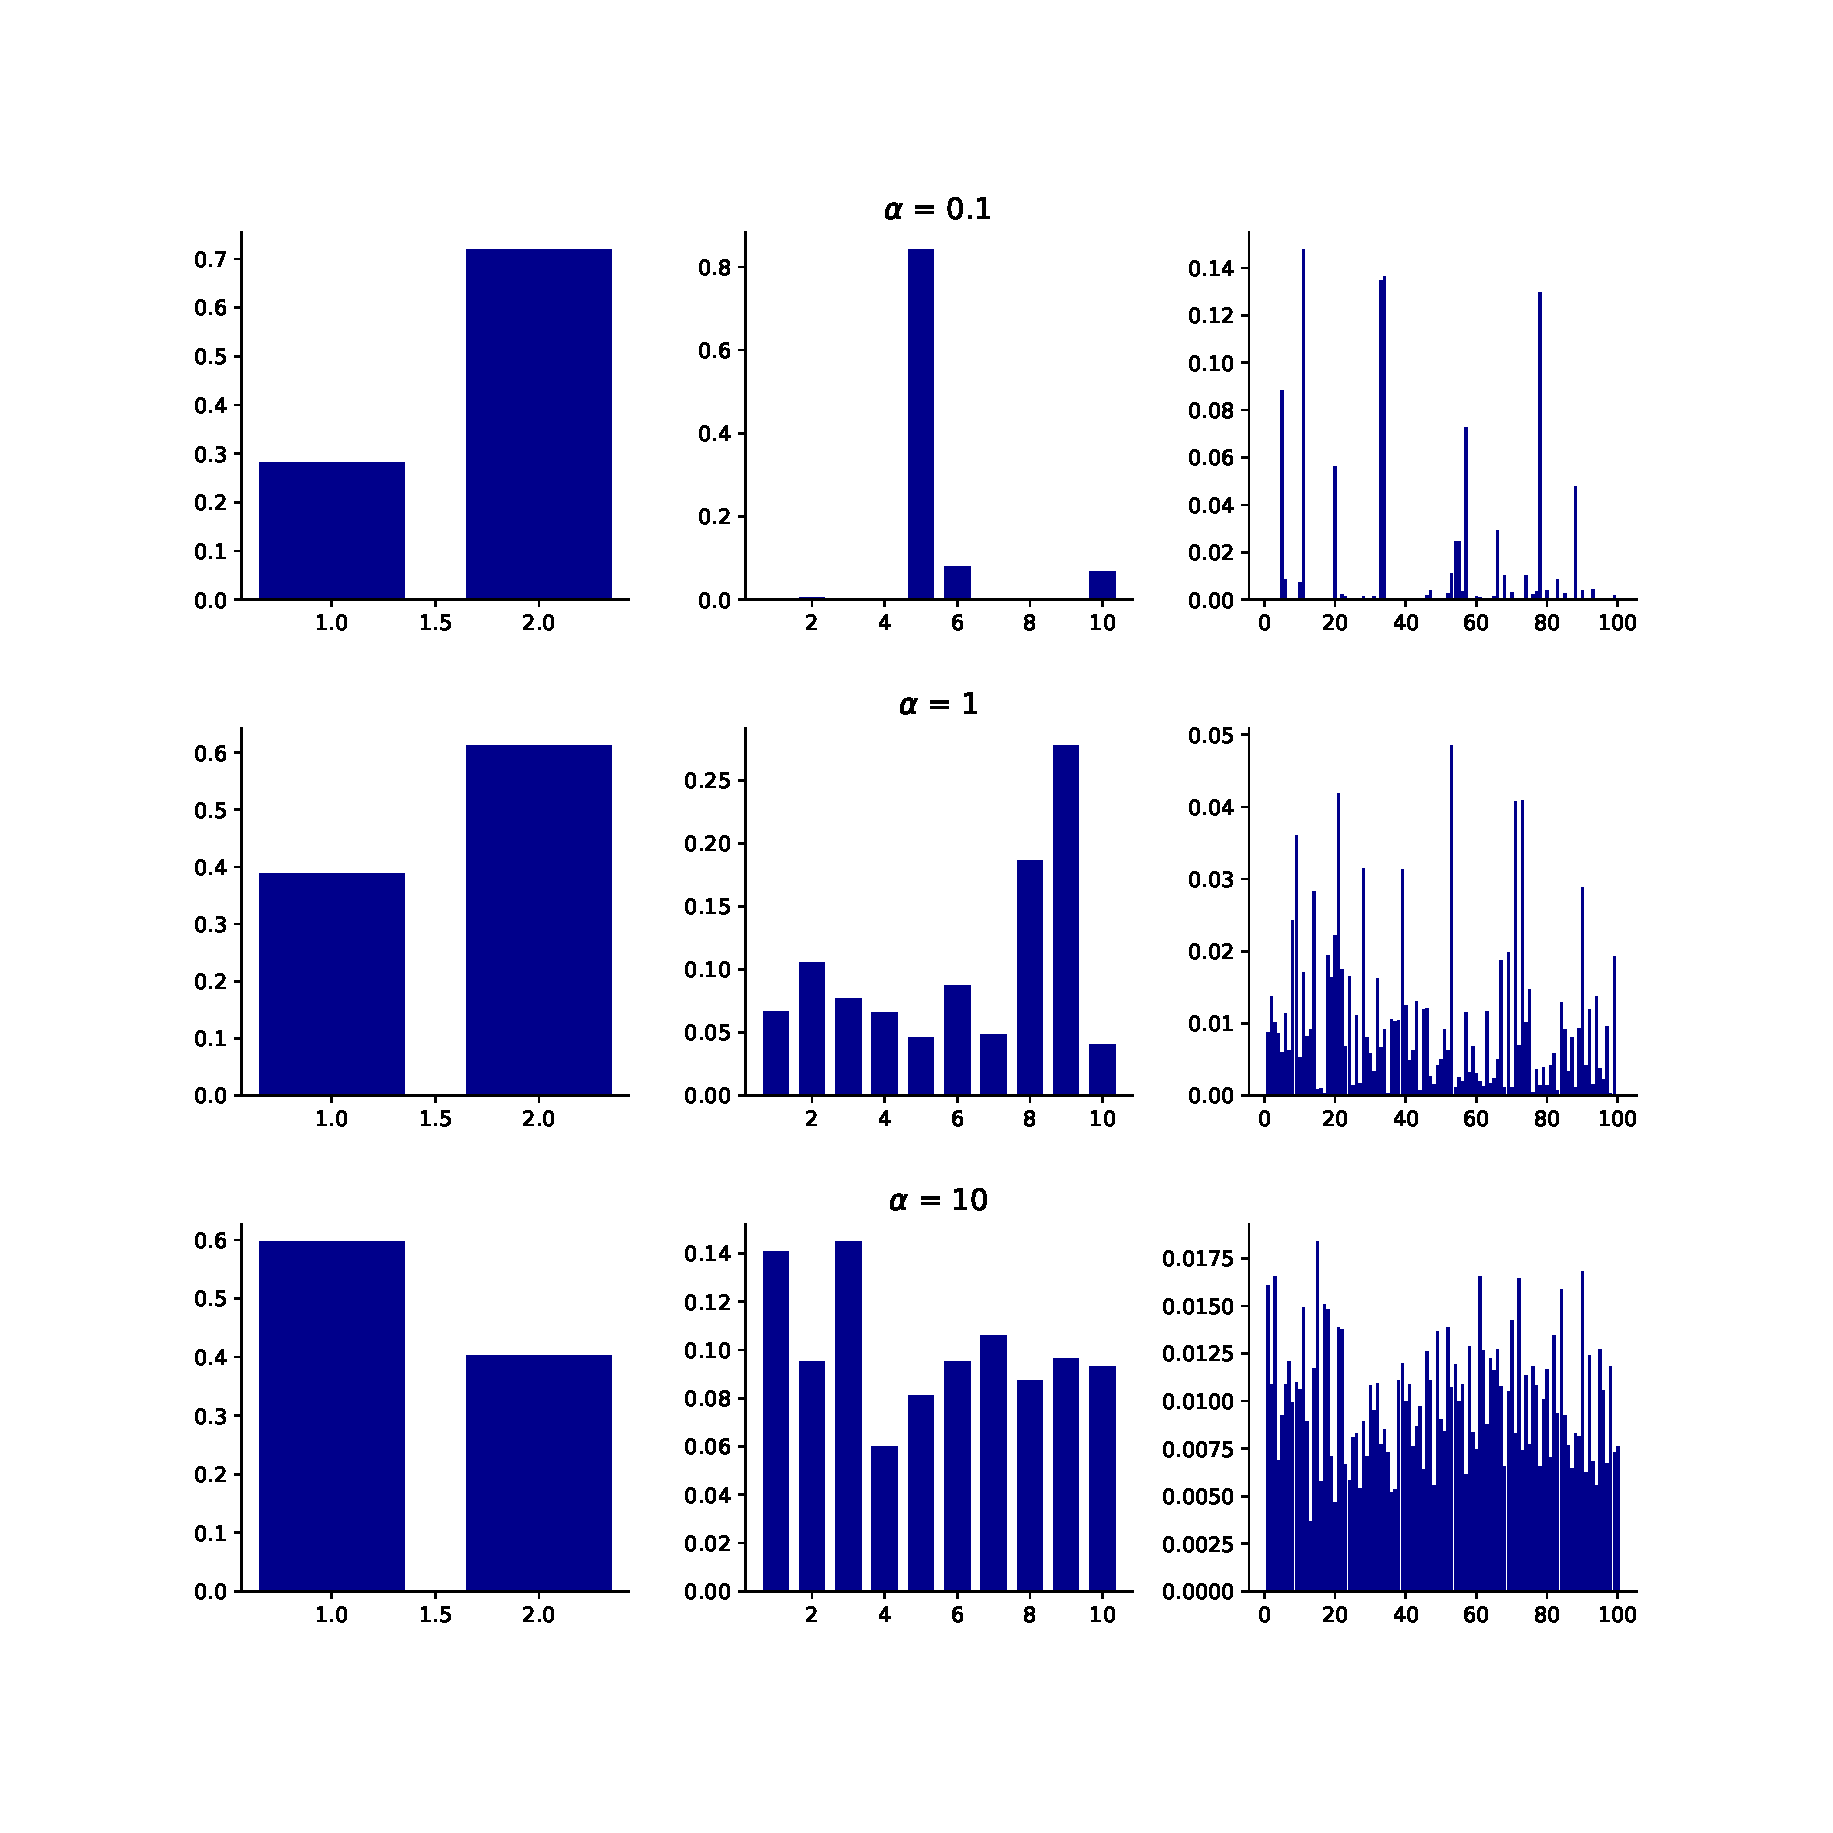
\includegraphics[width=\textwidth]{ch2/dirichlet_samples.eps}
    \caption{Muestra de una distribución Dirichlet simétrica con $\alpha \in \{0.1, 1, 10\}$ y $K\in\{2, 10, 100\}$.}
    \label{img:dirichlet_samples}
\end{figure}

\subsection{Dirichlet Process}
\label{sec:dp}

En un \textit{finite mixture model} se tiene $G(\phi) = \sum_{k=1}^{K} \pi_{k}\delta_{\phi_{k}}(\phi)$, luego al muestrear de $G$, con probabilidad uno se obtendrá exactamente $K$ \textit{clusters}. Sin embargo, es necesario tener un modelo más flexible, que pueda generar un número variable de \textit{clusters}. Una forma de hacer esto es remplazar la distribución discreta $G$ por una medida aleatoria de probabilidad, como el Dirichlet Process \citep{ferguson1973bayesian}, denotado $G\sim \text{DP}(\alpha, H)$.\\

Un \textbf{Dirichlet Process} (DP) es una distribución sobre medidas de probabilidad $G: \Phi \rightarrow \mathbb{R}^{+}$, donde $G(\phi)\geq 0$ y $\int_{\Phi}G(\phi)d\phi=1$. Un DP se define implícitamente por cumplir 

\begin{align}
    G(A_{1}), \ldots, G(A_{K}) \sim \text{Dir}(\alpha H(A_{1}), \ldots, \alpha H(A_{K}))
\end{align}

para cualquier partición finita $(A_{1}, \ldots, A_{k})$ de $\Phi$. En este caso, decimos que $G\sim \text{DP}(\alpha, H)$, donde $\alpha$ es llamado el \textbf{parámetro de concentración} y $H: \Phi \rightarrow \mathbb{R}^{+}$ es llamado la \textbf{medida base}.\\

Como $p(G(A_{1}), \ldots, G(A_{K}))$ es Dirichlet, la distribución marginal en cada partición distribuye beta $\text{Beta}(\alpha H(A_{i}), \alpha \sum_{j\neq i}H(A_{j}))$. El DP es considerado consistentemente definido, ya que si se particiona $\bar{A}_{1}$ en $A_{1}$ y $A_{2}$, entonces $G(\bar{A}_{1})$ y $G(A_{1})+G(A_{2})$ siguen la misma distribución beta. \\

Sea $\pi \sim \text{Dir}(\alpha)$, y $z|\pi  \sim \text{Cat}(\pi)$, si se integra $\pi$ afuera se obtiene la distribución predictiva del modelo Dirichlet-multinoulli:
\begin{align}
    z\sim \text{Cat}(\alpha_{1}/\alpha_{0}, \ldots, \alpha_{K}/\alpha_{0})
\end{align}
donde $\alpha_{0} = \sum_{k}\alpha_{k}$. Es decir, $p(z=k|\alpha)=\alpha_{k}/\alpha_{0}$. Ademas, la posterior de $\pi$ dada una observación viene dada por
\begin{align}
    \pi|z \sim \text{Dir}(\alpha_{1}+\mathbb{I}(z=1), \ldots, \alpha_{K}+\mathbb{I}(z=K))
\end{align}

El DP generaliza el resultado anterior a particiones arbitrarias. Si $G\sim \text{DP}(\alpha, H)$, luego $p(\phi \in A_{i})=H(A_{i})$ y la posterior es

\begin{align}
    p(G(A_{1}), \ldots, G(A_{K})|\phi, \alpha, H) = \text{Dir}(\alpha H(A_{1})+\mathbb{I}(\phi \in A_{1}), \ldots, \alpha H(A_{K})+\mathbb{I}(\phi \in A_{K}))
\end{align}

Esto se mantiene para cualquier conjunto de particiones. Por lo tanto, si observamos multiples muestras $\bar{\phi}_{1:N}\sim G$, la nueva posterior está dada por 

\begin{align}
G|\bar{\phi}_{1:N}, \alpha, H \sim \text{DP}\bigg(\alpha+N, \frac{1}{\alpha+N}\bigg(\alpha H+\sum_{i=1}^{N}\delta_{\bar{\phi}_{i}}\bigg)\bigg)
\end{align}

Por ende el DP define un \textit{prior} conjugado para cualquier espacio medible, donde el parámetro de concentración $\alpha$ es el tamaño de muestro efectivo de la medida base $H$.\\

Existen diferentes perspectivas que ayudan a entender la propiedad de \textit{clustering} de un Dirichlet Process. En la sección \ref{sec:sbp}. y \ref{sec:crp}. se describen dos: el Stick Breaking Process y Chinese Restaurant Process (CRP).

\subsection{Stick Breaking Process}
\label{sec:sbp}

En esta sección se describe una definición constructiva de un DP, conocida como \textit{stick breaking process} \citep{sethuraman1994constructive}. Sea $\pi=\{\pi_{k}\}_{k=1}^{\infty}$ una mezcla de pesos infinita derivada a partir del siguiente proceso:
\begin{align}
    \beta_{k} & \sim \text{Beta}(1, \alpha)\\
    \pi_{k} & = \beta_{k}\prod_{l=1}^{k-1}(1-\beta_{l}) = \beta_{k}(1-\sum_{l=1}^{k-1}\pi_{l})
\end{align}

Esto se suele denotar como $\pi \sim \text{GEM}(\alpha)$, donde GEM representa Griffiths, Engen y McCloskey, ver Figura  \ref{img:stick_breaking} para una ilustración. 

\begin{figure}
    \centering
    \includegraphics[width=0.6\textwidth]{ch2/stick_breaking.png}
    \caption{Ilustración de \textit{stick breaking process}. Se tiene una barra de largo 1, la cual se rompe en un punto aleatorio $\beta_{1}$, el largo de la pieza restante es llamada $\pi_{1}$, luego recursivamente se rompe la barra restante, así generando $\pi_{2}, \pi_{3}, \ldots$. Fuente: Figura 2.22 de \citep{sudderth2006graphical}.}
    \label{img:stick_breaking}
\end{figure}

Algunos ejemplos de este proceso son mostrados en la Figura \ref{img:dp_samples} (a). A mayor $\alpha$, menos varianza y mayor número de átomos, por el contrario, pequeños valores de $\alpha$ muestran una alta varianza y menor número de átomos. Se puede demostrar que este proceso termina con probabilidad uno, a pesar que el número de elementos que genera incrementa con $\alpha$. Además, el tamaño del componente $\pi_{k}$ decrece en promedio. La distribución $G$ se puede definir como sigue:

\begin{align}
    G(\phi) = \sum_{k=1}^{\infty}\pi_{k}\delta_{\phi_{k}}(\phi)
\end{align}
 
, donde $\pi \sim \text{GEM}(\alpha)$ y $\phi_{k} \sim H$. Es posible demostrar que $G \sim \text{DP}(\alpha, H)$. Como consecuencia de esta construcción, las muestras de un DP son \textbf{discretas con probabilidad uno}. En otras palabras, al muestrear $\bar{\phi_{i}}\sim G$ se observarán valores repetidos, por lo que la mayoría de los datos vendrán de los $\phi_{k}$ con $\pi_{k}$ más largos. En la Figura \ref{img:dp_samples} (b) se muestra un par de medidas aleatorias generadas a partir de un DP con una medida base normal.\\

\begin{figure}
    \centering
    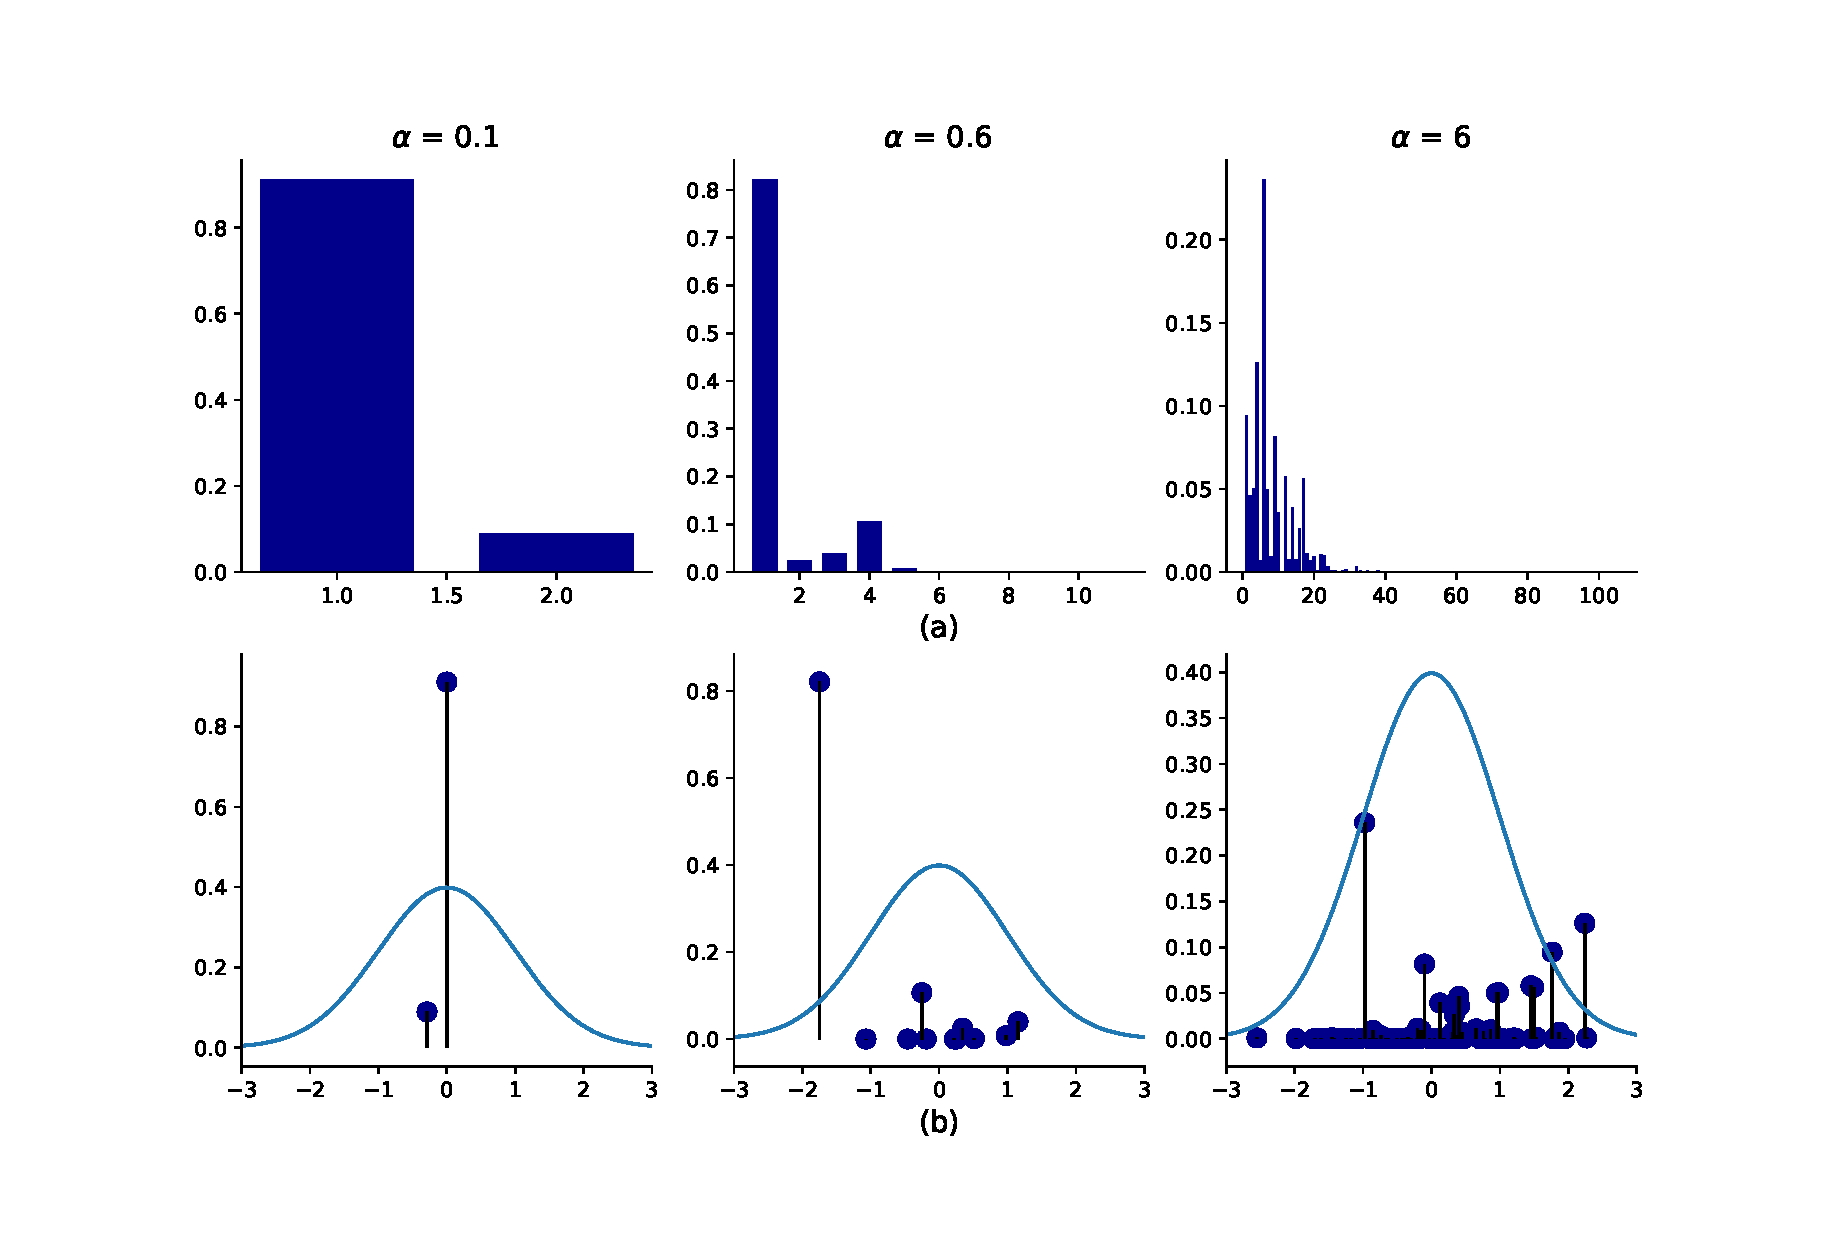
\includegraphics[width=\textwidth]{ch2/dp_samples.eps}
    \caption{(a) Muestras de una distribución GEM con parámetros de concentración $\alpha\in \{0.1, 0.6, 6\}$. (b) Medidas aleatorias generadas a partir de un Dirichlet Process con medida base normal $\mathcal{N}(0,1)$ con parámetros de concentración $\alpha\in \{0.1, 0.6, 6\}$}
    \label{img:dp_samples}
\end{figure}

\subsection{Chinese Restaurant Process}
\label{sec:crp}

Trabajar con infinitos átomos puede ser bastante problemático. Para sortear esta dificultad se puede explotar la propiedad de \textit{clustering} de un DP. Sea $\bar{\phi}_{1:N}\sim G$ observaciones generadas a partir de $G\sim \text{DP}(\alpha, H)$, sea $K$ los distintos valores de $\bar{\phi}_{1:N}$, luego la distribución predictiva condicionada en las $N$ observaciones está dada por

\begin{align}
p(\bar{\phi}_{N+1}=\phi|\bar{\phi}_{1:N}, \alpha, H) = \frac{1}{\alpha+N}\bigg(\alpha H(\phi)+\sum_{k=1}^{K}N_{k}\delta_{\bar{\phi}_{k}}(\phi)\bigg)
\end{align}

donde $N_{k}$ es el número de observaciones previas iguales a $\phi_{k}$. Este esquema de muestreo es llamado \textit{Polya urn} o \textit{Blackwell-MacQueen}. \\

Es más conveniente trabajar con variables discretas $z_{i}$ que especifican cual $\phi_{k}$ usar, así, se define $\bar{\phi}_{i}=\phi_{z_{i}}$. En base a esta expresión se tiene lo siguiente:

\begin{align}
p(z_{N+1}=z|z_{1:N}, \alpha) = \frac{1}{\alpha+N}\bigg(\alpha\mathbb{I}(z=k^{*})+\sum_{k=1}^{K}N_{k}\mathbb{I}(z=k)\bigg)
\end{align}

, donde $k^{*}$ representa un nuevo \textit{cluster} que no ha sido usado aún. Este proceso es denominado Chinese Restaurant Process (CRP) \citep{aldous1985exchangeability}, basado en la oferta aparentemente infinita de mesas en ciertos restaurantes Chinos. La analogía es la siguiente: Las tablas del restaurante son los \textit{clusters}  y los clientes son las observaciones. Cuando una persona entra al restaurante, esta puede escoger sentarse en una tabla existente con probabilidad proporcional al número de personas ya sentadas en esa tabla ($N_{k}$), en otro caso, con una probabilidad decreciente a medida que más personas entran al restaurante (debido a $1/(\alpha +N))$ escogerá sentarse en una nueva tabla $k^{*}$. El resultado de este proceso es una distribución sobre particiones de los naturales, la cual es como una distribución de clientes a tablas.\\

El hecho de que las tablas actualmente ocupadas son más probables de obtener nuevos clientes se suele llamar el fenómeno del \textit{rich get richer}. En efecto, se puede demostrar que la distribución del número de \textit{clusters} que induce este \textit{prior} es básicamente una ley de potencia, donde el número de tablas $K$ con probabilidad 1 se aproxima a $\alpha log(N)$ cuando $N\rightarrow \infty$, mostrando que la complejidad del modelo crece logarítmicamente con el tamaño de los datos.

\section{Modelos de tópicos}
\label{sec:topic_models}
Los modelos de tópicos probabilísticos ayudan a descubrir los temas latentes (\textit{clusters}) en una colección de documentos, como estos temas están conectados unos a otros y cómo cambian en el tiempo. Permiten resumir un gran colección de documentos a través de sus temas y organizarlos entorno a estos.\\

Los modelos probabilísticos tratan un tópico como una distribución de probabilidad discreta sobre el vocabulario del corpus, siendo un práctica habitual interpretar un tópico a partir de sus $N$ palabras más probables. Por ejemplo, con $N=5$ las palabras más probables de un tópico son: \quotes{llaves}, \quotes{domicilio}, \quotes{individuos}, \quotes{casa} y \quotes{porton}, por lo que una etiqueta valida para este tópico podría ser \quotes{portonazo}.\\ 

En \textit{procesamiento del lenguaje natural} (NLP) se suele trabajar bajo la asumpción de \textbf{bag of words} (bolsa de palabras), es decir, tanto los documentos como las palabras son tratadas como intercambiables. Es importante hacer notar que itercambiabilidad no es equivalente a que las variables aleatorias son independientes e identicamente distribuidas. Más bien, intercambiabilidad esencialmente puede ser interpretado como condicionalmente independientes e identicamente distribuidas, donde el condicionamiento es con respecto a los parámetros de una distribución de probabilidad. Por lo tanto, el supuesto de intercambiabilidad es claramente un supuesto de simplificación cuya principal justificación es la construcción de algoritmos computacionales más eficientes.\\

Un \textit{mixture model} que trabaja bajo la asumpción de \textit{bag of words} es \textit{mixture of unigrams} \citep{nigam2000text}, el cual asume que todos los documentos provienen de un solo \textit{cluster} dentro de un conjunto finito de $K$ \textit{clusters}. Los documentos de un \textit{cluster} discuten solo un tópico particular $z$, y cada tópico $z$ está asociado a una distribución categórica. Así, la verosimilitud de observar un documento $d$ es

\begin{align}
    w|z &\sim \text{Cat}(\theta_{z})\\
    p(w_{1}, \ldots, w_{N_{d}}) &= \sum_{z=1}^{K}p(z)\prod_{i=1}^{N_{d}}p(w_{i}|z)
\end{align}

En las secciones \ref{sec:lda}-\ref{sec:hdp} se describe en detalle dos modelos de tópicos probabilísticos, Latent Dirichlet Allocation (LDA) y Hierarchical Dirichlet Process (HDP), considerado la generalización no parámetrica de LDA, donde el número de tópicos a descubrir no está acotado y se infiere a partir del corpus.\\

En comparación a \textit{mixture of unigrams}, LDA y HDP suponen que las palabras de un documento provienen de un mismo \textit{mixture model}, donde a nivel corpus los \textit{mixture models} comparten parámetros, que vienen siendo los tópicos, pero las \textit{mixtures of topics} son específicas de cada documento. Esto permite relajar la asumpción de que cada documento es generado por un solo tópico, debido a que cada palabra proviene de algún tópico, por lo que un documento puede tener presencia de más de un tema.\\

\subsection{Latent Dirichlet Allocation}
\label{sec:lda}

En Latent Dirichlet Allocation (LDA) \citep{blei2003latent} cada tópico es una distribución de probabilidad sobre un vocabulario fijo $V$. Cada documento $d$ tiene su propia mezcla de tópicos $\pi_{d}$. La asignación $z_{d,n}\in\{1, \ldots, K\}$  de de una palabra $n$ a un tópico $z$ es dibujada a partir de $\pi_{d}$. El modelo completo es como sigue

\begin{align}
    \phi_{k}|\eta \quad & \sim\quad \text{Dir}(\frac{\eta}{|V|}1_{|V|})\\
    \pi_{d}|\alpha \quad & \sim \quad \text{Dir}(\frac{\alpha}{K}1_{K})\\
    z_{d,n}|\pi_{d} \quad & \sim \quad \text{Cat}(\pi_{d})\\
    w_{d,n}|z_{d,n}, \phi_{1:K} \quad & \sim \quad \text{Cat}(\phi_{z_{d,n}})
\end{align}

Esto es ilustrado en la Figura \ref{img:lda}.
\begin{figure}
  \centering
  \tikz{ %

    \node[latent, dashed] (alpha) {$\alpha$} ; %
    \node[latent, right=of alpha] (pi) {$\pi_{d}$} ; %
    \node[latent, right=of pi] (z) {$z_{d,n}$} ; %
    \node[obs, right=of z] (w) {$w_{d,n}$}   ; %
    \node[latent, right=of w] (phi) {$\phi_{k}$} ; %
    \node[latent, right=of phi, dashed] (eta) {$\eta$} ;%
    \plate[inner sep=0.25cm, xshift=-0.12cm, yshift=0.12cm] {plate1} {(z) (w)} {$N_{d}$}; %
    \plate[inner sep=0.25cm, xshift=-0.12cm, yshift=0.12cm] {plate2} {(pi) (plate1)} {$D$}; %
    \plate[inner sep=0.25cm, xshift=-0.12cm, yshift=0.12cm] {plate3} {(phi)} {$K$}; %
    \edge {alpha} {pi} ; %
    \edge {pi} {z} ; %
    \edge {z,phi} {w} ; %
    \edge {eta} {phi} ; %
  }
\caption{Representación gráfica de LDA: círculos denotan variables aleatorias, círculos abiertos denotan parámetros, círculos sombreados denotan variables observadas y los platos indican replicación.}
\label{img:lda}
\end{figure}

La probabilidad conjunta del modelo:
\begin{equation}
    p(\phi, \pi, z, w|\alpha, \eta)= \prod_{k=1}^{K}p(\phi_{k}|\eta)\prod_{d=1}^{D}p(\pi_{d}|\alpha)\prod_{n=1}^{N_{d}}p(z_{n,d}|\pi_{d})p(w_{d,n}|\phi_{1:K}, z_{d,n})
\end{equation}

La distribución a posterior:
\begin{equation}
    p(\phi, \pi, z|w, \alpha, \eta) = \frac{p(\phi, \pi, z, w|\alpha, \eta)}{p(w|\alpha, \eta)}
\end{equation}

La distribución posterior es computacionalmente intratable para inferencia exacta, debido a que para normalizar la distribución se debe marginalizar sobre todas las variables ocultas y escribir la constante de normalización en términos de los parámetros del modelo. Para poder computar la posterior es necesario utilizar algoritmos de inferencia aproximada, donde el enfoque habitual es Markov Chain Monte Carlo (MCMC) \citep{andrieu2003introduction} e Inferencia Variacional (VI) \citep{blei2017variational}. En \citep{blei2003latent} se propone un algoritmo basado en VI y en \citep{griffiths2004finding} en MCMC.\\

Una representación equivalente en LDA sería generar cada palabra de un documento $d$ a partir de un tópico dibujado por una distribución $G_{d}$,

\begin{align}
    \phi_{k}|\eta \quad & \sim \quad \text{Dir}(\frac{\eta}{|V|}1_{|V|})\\
    \pi_{d}|\alpha \quad & \sim \quad \text{Dir}(\frac{\alpha}{K}1_{K})\\
    G_{d}(\phi)\quad & = \quad \sum_{k=1}^{K}\pi_{d, k}\delta_{\phi_{k}}(\phi)\\
    \phi_{d,n}|\pi_{d}, \phi_{1:K} \quad & \sim \quad G_{d}\\
    w_{d,n}|\phi_{d,n} \quad & \sim \quad  \text{Cat}(\phi_{d,n})
\end{align}

\subsection{Hierarchical Dirichlet Process}
\label{sec:hdp}

Hierarchical Dirichlet Process (HDP)\citep{teh2005sharing} es un \textit{prior} jerárquico no paramétrico, el cual está formado por un DP cuya medida base $G_{0}$ es dibujada a partir de un DP. En el caso de modelamiento de tópicos, se tiene un medida global $G_{0}$ a nivel corpus que es dibujada a partir de un DP con medida base Dirichlet y una medida $G_{d}$ para cada documento que es dibujada a partir de un DP con medida base $G_{0}$. El modelo completo es como sigue

\begin{align}
   H \quad &= \quad \text{Dir}(\frac{\eta}{|V|}1_{|V|})\\
   G_{0}|\gamma, H \quad &\sim \quad \text{DP}(\gamma, H)\\
   G_{d}|\alpha, G_{0} \quad &\sim \quad \text{DP}(\alpha_{0}, G_{0})\\
   \phi_{d,n}|G_{d} \quad &\sim \quad G_{d}\\
   w_{d,n}|\phi_{d,n} \quad &\sim \quad \text{Cat}(\phi_{d,n})
\end{align}

Esto es ilustrado en la Figura \ref{img:hdp}.

\begin{figure}
  \centering
  \tikz{ %
    \node[latent, dashed] (H) {$H$} ; %
    \node[latent, right=of H] (G0) {$G_{0}$} ; %
    \node[latent, above= of G0, dashed] (gamma) {$\gamma$} ; %
    \node[latent, right=of G0] (Gd) {$G_{d}$} ; %
    \node[latent, above= of Gd, dashed] (alpha0) {$\alpha_{0}$} ; %
    \node[latent, right= of Gd] (phi) {$\phi_{d,n}$} ; %
    \node[obs, right=of phi] (w) {$w_{d,n}$}   ; %
    \plate[inner sep=0.25cm, xshift=-0.12cm, yshift=0.12cm] {plate1} {(phi) (w)} {$N_{d}$}; %
    \plate[inner sep=0.25cm, xshift=-0.12cm, yshift=0.12cm] {plate2} {(Gd) (plate1)} {$D$}; %
    \edge {H, gamma} {G0} ; %
    \edge {G0, alpha0} {Gd} ; %
    \edge {Gd} {phi} ; %
    \edge {phi} {w} ; %
  }
\caption{Representación gráfica de HDP: círculos denotan variables aleatorias, círculos abiertos denotan parámetros, círculos sombreados denotan variables observadas y los platos indican replicación.}
\label{img:hdp}
\end{figure}

La discretitud a nivel corpus de $G_{0}$ asegura que todos los documentos comparten el mismo conjunto de tópicos (\textit{mixture components}). A nivel documento $G_{d}$ hereda los tópicos de $G_{0}$, pero los pesos de cada tópico (\textit{mixture proportions}) es específica del documento.\\


\subsubsection{Stick Breaking Construction}
Aplicando \textit{stick breaking construction} se tiene que para el DP dibujado a nivel corpus la siguiente representación:

\begin{align}
    \beta_{k}^{'} \quad &\sim \quad \text{Beta}(1, \gamma) \\
    \beta_{k} \quad &= \quad \beta_{k}^{'}\prod_{l=1}^{k-1}(1-\beta_{l}^{'})\\
    \phi_{k} \quad &\sim \quad H  \\
    G_{0}(\phi) \quad &= \quad \sum_{k=1}^{\infty}\beta_{k}\delta_{\phi_{k}}(\phi)
\end{align}

Así, $G_{0}$ es discreto y tiene soporte en los átomos $\phi = \{\phi\}_{k=1}^{\infty}$ con pesos $\beta=\{\beta_{k}\}_{k=1}^{\infty}$, siendo la distribución de $\beta$ escrita como $\beta \sim \text{GEM}(\gamma)$. La construcción a nivel documento de $G_{d}$ es:

\begin{align}
    \pi_{d,k}^{'} \quad &\sim \quad \text{Beta}\big(\alpha_{0}\beta_{k}, \alpha_{0}\big(1-\sum_{l=1}^{k}\beta_{l}\big)\big)\\
    \pi_{d,k} \quad &= \quad \pi_{d,k}^{'}\prod_{l=1}^{k-1}(1-\pi_{d,l}^{'})\\
    G_{d}(\phi) \quad &= \quad\sum_{k=1}^{\infty}\pi_{d,k}\delta_{\phi_{k}}(\phi)\\
    \phi_{d,n}|\pi_{d}, \phi_{1:\infty} \quad &\sim \quad G_{d}
\end{align}

Donde $\phi = \{\phi_{k}\}_{k=1}^{\infty}$ son los mismos átomos de $G_{0}$. Esto es ilustrado en la Figura \ref{img:hdp_sbc}.

%stick breaking
\begin{figure}
  \centering
  \tikz{ %
    \node[latent] (beta) {$\beta$} ; %
    \node[latent, above= of beta, dashed] (gamma) {$\gamma$} ; %
    \node[latent, right=of beta] (pi) {$\pi_{d}$} ; %
    \node[latent, above= of pi, dashed] (alpha0) {$\alpha_{0}$} ; %
    \node[latent, right= of pi] (z) {$z_{d,n}$} ; %
    \node[obs, right=of z] (w) {$w_{d,n}$}   ; %
    \node[latent, right=of w] (phi) {$\phi$} ; %
    \node[latent, above=of phi, dashed] (H) {$H$} ; %
    \plate[inner sep=0.25cm, xshift=-0.12cm, yshift=0.12cm] {plate1} {(z) (w)} {$N_{d}$}; %
    \plate[inner sep=0.25cm, xshift=-0.12cm, yshift=0.12cm] {plate2} {(pi) (plate1)} {$D$}; %
    \plate[inner sep=0.25cm, xshift=-0.12cm, yshift=0.12cm] {plate3} {(phi)} {$K (\infty)$}; %
    \edge {gamma} {beta} ; %
    \edge {beta, alpha0} {pi} ; %
    \edge {pi} {z} ; %
    \edge {z, phi} {w} ; %
    \edge {H} {phi} ; %
  }
\caption{Representación gráfica de la construcción stick-breaking de HDP: círculos denotan variables aleatorias, círculos abiertos denotan parámetros, círculos sombreados denotan variables observadas y los platos indican replicación.}
\label{img:hdp_sbc}
\end{figure}

\subsubsection{Chinese Restaurant Franchise Process}

Una construcción alternativa de HDP es conocida bajo el nombre de \textit{Chinese Restaurant Franchise Process} (CRF), una extensión del CRP, que permite compartir un conjunto de platos a través de una cadena de restaurantes Chinos. La analogía es la siguiente, se tienen $D$ restaurantes, cada uno con $N_{d}$ clientes que se sientan en tablas $t_{d,i}$, en cada tabla es servido un único plato $\phi_{k}\sim H$ a partir de un menú común para todos los restaurantes. \\

Sea $m_{dk}$ el número de tablas sirviendo el plato $k$ en el restaurante $d$, así $m_{d.}$ representa el número de tablas en el restaurante $d$, $m_{.k}$ representa el número de tablas sirviendo el plato $k$, y $m_{..}$ el número total de tablas ocupadas. Al integrar $G_{d}$ la probabilidad condicional del cliente $i$-ésimo este en la tabla $t$ se puede escribir como sigue:

\begin{align}
p(t_{di}=t|t_{d1}, \ldots, t_{d,i-1}, \alpha_{0}, G_{0}) = \frac{1}{\alpha_{0}+i-1}\bigg(\alpha_{0}\mathbb{I}(t=t^{*})+\sum_{t^{'}=1}^{m_{d.}}N_{dt^{'}}\mathbb{I}(t=t^{'})\bigg)
\end{align}

donde $N_{dt^{'}}$ representa los clientes del restaurante $d$ que están sentados en la tabla $t^{'}$. Con probabilidad proporcional a los clientes sentados en la tabla $t$ los clientes del restaurante se sentarán en esta y con probabilidad proporcional a $\alpha_{0}$ en una nueva. Una vez todos los clientes estan sentados se tiene una partición sobre $\phi_{d1}, \ldots, \phi_{dN_{d}}$ para cada documento $d$. Luego, al integrar afuera $G_{0}$ se obtiene:

\begin{align}
    p(z_{dt}=z|z_{11}, z_{12}, \ldots, z_{d1}, \ldots, z_{d, t-1}|\gamma, H) = \frac{1}{\gamma+m_{..}}\bigg(\gamma\mathbb{I}(z=k^{*})+\sum_{k=1}^{K}m_{.k}\mathbb{I}(z=k)\bigg)
\end{align}

en este caso se tiene que la tabla $t$ del restaurante $d$ con probabilidad proporcional al número de tablas que sirven el plato $k$ ($m_{.k}$) servirá el plato $k$ y con probabilidad proporcional a $\gamma$ servirá un nuevo plato.\\

Por último, al igual que LDA la distribución posterior de HDP es intratable, por lo que se debe recurrir a técnicas de inferencia aproximada. En \citep{teh2005sharing} se propone un algoritmo basado en MCMC bajo la construcción CRF de un HDP. 

\section{Modelamiento de la evolución de los tópicos en el tiempo}
\label{sec:topic_evolution} 

En \citep{wilson2011tracking} y \citep{beykikhoshk2018discovering} se propone una metodología que permite capturar los dinámismos mencionados usando LDA y HDP respectivamente. Donde se propone dividir el corpus en $T$ épocas, en cada época se entrena un modelo de tópicos estático, obteniéndose así $T$ conjuntos de tópicos $\phi=\{\phi_{1}, \ldots, \phi_{T}\}$, con $\phi_{t}=\{\phi_{t,1}, \ldots, \phi_{t,K_{t}}\}$ el conjunto de tópicos que describen la época $t$, y $K_{t}$ el número de tópicos inferido en esa época. Una vez descubiertos los tópicos se hace uso de medidas de distancia o similitud para relacionar tópicos de épocas adyacentes.\\

En las secciones \ref{sec:similarity_graph}-\ref{sec:automatic_construction} se describe la metodología propuesta en \citep{beykikhoshk2018discovering} para relacionar los tópicos descubiertos de épocas adyacentes.

\subsection{Gráfo de similitud temporal}
\label{sec:similarity_graph}
Para relacionar los tópicos de una época es necesario contar una medida de similitud $\rho \in [0,1]$, con esta médida de similitud se puede construir un gráfo, donde los nodos son los tópicos de una época y los arcos relacionan tópicos de una época con la siguiente, siendo el peso del arco la similitud entre los tópicos. Una vez construido el grafo se eliminan las conexiones débiles en base a un umbral $\zeta \in [0,1]$ a definir, reteniendo solo aquellas conexiones entre tópicos suficientemente similares entre épocas adyacentes, matemáticamente se poda el arco entre los tópicos $\phi_{t,i}$ y $\phi_{t+1,j}$ si $\rho(\phi_{t,i}, \phi_{t+1,j})\leq \tau.\\

Está metodología permite detectar desaparición de un tópico, nacimiento de un nuevo tópico, como también división o fusión entre diferentes tópicos. A continuación se define en detalle cada uno de estos dinamismos:

\begin{itemize}
    \item \textbf{Nacimiento de un tópico:} Si un tópico no tiene ningún arco entrante, por ejemplo, en la Figura \ref{img:graph} el tópico $\phi_{j+2}$ en $t$.
    \item \textbf{Muerte de un tópico:} Si un tópico no tiene ningún arco saliente, por ejemplo, en la Figura \ref{img:graph} el tópico $\phi_{j}$ en $t$.
    \item \textbf{Evolución de un tópico:} Cuando un tópico tiene exactamente un arco de entrada y salida, por ejemplo, en la Figura \ref{img:graph} entre las épocas $t$ y $t+1$ se tiene que el tópico $\phi_{j+2}$ evoluciona del tópico $\phi_{k+1}$.
    \item \textbf{División de un tópico:} Si un tópico tiene más de un arco saliente, por ejemplo, en la Figura \ref{img:graph} el tópico $\phi_{i}$ de $t-1$ se divide en $t+1$ en los tópicos $\phi_{j}$ y $\phi_{j+1}$.
    \item \textbf{Fusión de un tópico:} Cuando un tópico tiene más de un arco entrante, este tipo de tópicos también pueden ser entendidos como un nuevo tópico, por ejemplo, en la Figura \ref{img:graph} los tópicos $\phi_{i}$ y $\phi_{i+1}$ de $t-1$ forman al tópico $\phi_{j+1}$ en $t$.
\end{itemize}

\begin{figure}
    \centering
    \includegraphics[width=0.8\textwidth]{ch2/similarity_graph.png}
    \caption{Ilustración conceptual del grafo de similitud que modela la dinámica de los tópicos en el tiempo. Un nodo corresponde a un tópico en una época específica; el ancho de los arcos es proporcional a la similitud entre los tópicos, arcos ausentes fueron eliminados por presentar una similitud menor a un umbral. Fuente:  Figura 3 de \citep{beykikhoshk2018discovering}}
    \label{img:graph}
\end{figure}

\subsection{Construcción automática del grafo de similitud}
\label{sec:automatic_construction}

Un aspecto relevante de esta metodología es definir el úmbral de corte, el cual no es fácilmente interpretable, además el úmbral depende de la médida de similitud escogida, dificultando así la comparación entre médidas de similitud. En \citep{beykikhoshk2018discovering} proponen una alternativa más interpretable para definir el úmbral, para esto estiman la función de densidad acumulada (cdf) del grafo inicial, donde todos los nodos de una época están conectados con todos los nodos de la época adyacente, al que de ahora en adelante se denota grafo \textit{fully-connected}. \\

Sea $F_{p}$ la cdf sobre las similitudes del grafo inicial, luego sea $\zeta \in [0,1]$ el punto operante de la cdf, luego se elimina el arco entre los tópicos $\phi_{t,i}$ y $\phi_{t+1,j}$ si $\rho(\phi_{t,i}, \phi_{t+1,j})\leq F_{p}^{-1}(\zeta)$, donde  $F_{p}^{-1}(\zeta)$ es el cuantil $\zeta$ de $F_{p}$. En \ref{img:cdf_sim} se tiene una ilustración para tres médidas de similitud, en esta se observa que la elección arbitraria del úmbral de corte depende fuertemente de la médida de similitud escógida, por lo que la elección en base a la cdf puede ser más apropiada.

\begin{figure}
    \centering
    \includegraphics[width=0.8\textwidth]{ch2/cdf_sim.png}
    \caption{Estimación empírica de la función de densidad acumulada (cdf) de la similitud entre tópicos de épocas adyacentes en un grafo \textit{fully-connected} para tres medidas de similitud. Fuente: Figura 4 \citep{beykikhoshk2018discovering}.}
    \label{img:cdf_sim}
\end{figure}


\chapter{Metodología}
\label{ch:methodology}
En este capítulo se describe la metodología propuesta para el descubrimiento de tópicos y su evolución en el tiempo. En primer lugar, en la sección \ref{sec:processing} se describe la metodología de procesamiento utilizada para limpiar los datos que usa el modelo. En segundo lugar, en la sección \ref{sec:model_selected} se justifica la elección del modelo de tópicos. En tercer lugar, en la sección \ref{sec:build_graph} se describe la metodología escogida para modelar la evolución en el tiempo y la médida de similitud utilizada para comparar tópicos de épocas adyacentes. En cuarto lugar, en la sección \ref{sec:hiperparameters} se describen los hiperparámetros y su configuración. Por último, en la sección \ref{sec:methodology_resume} se resume de manera global la metodología.

\section{Procesamiento}
\label{sec:processing}

El propósito del procesamiento es simplificar eliminar el ruido en los datos y a su vez mantener el \textit{core} de palabras del corpus. En el caso del modelamiento de tópicos, esta etapa puede reducir significativamente el vocabulario. Como consecuencia, esto puede traer una mejora en la significancia estadística de los modelos, puesto que se puede obtener un mejor balance entre cantidad de parámetros y observaciones. Adicionalmente, puede facilitar la interpretación de los tópicos, removiendo palabras que aportan poca información.\\

En este experimento se aplicaron las siguientes cinco etapas:
\begin{enumerate}
  \item \textbf{Tokenización}: La tokenización es una operación sobre una cadena de caracteres (\textit{string}) que consiste en dividir el \textit{string} en un conjunto de términos (ej: en base al caracter espacio), obteniéndose así una lista de elementos llamados \textit{tokens}, que en términos simples pueden considerarse como palabras.
\item \textbf{Procesamiento de caracteres}: En esta etapa se suelen aplicar algunas operaciones básicas de procesamiento. En este proceso se llevan los tokens a unicode y minúsculas. Luego, se eliminan patrones de caracteres que difícilmente pueden tener algún significado, como correos electrónicos, símbolos de puntuación, tokens con números y letras o solo números. 
\item \textbf{Eliminación de stopwords}: Las \textit{stopwords} \citep{wilbur1992automatic} son palabras que aportan poca información (ej: artículos, preposiciones y conectores), usualmente tienen un alta frecuencia dentro del corpus. Para esto se utiliza una lista de palabras disponibles en el paquete NLTK de Python, el cual contiene 313 palabras \citep{bird2009natural}. Además, esta lista es alimentada con 951 \textit{stopwords} contextuales que corresponden a palabras específicas del corpus que aportan poca información. En el caso del robo de vehículos palabras relacionas a \quotes{robo} o \quotes{vehículo} no aportan ninguna información, puesto a que todos los relatos hablan del robo de un vehículo. 
\item \textbf{Filtro por vocabulario}: Con el propósito de mantener palabras \quotes{humanamente legibles} se utiliza un vocabulario. Para esto se utiliza el vocabulario del corpus SUC que se describe en la sección \ref{sec:word_embeddings}, de esta manera toda palabra tiene su \textit{word embedding}. 
\item \textbf{Filtro por frecuencia}: En este nivel se eliminan los \textit{tokens} con baja frecuencia, dado que un modelo difícilmente aprenderá algún patrón de un evento que tiene muy pocas realizaciones, menos si tiene una realización única. Esta etapa se aplica a nivel época, eliminando aquellos tokens que aparecen en menos del 0.1\% de los documentos de su respectiva época.
\item \textbf{Eliminación de documentos}: En el último nivel se eliminan aquellos documentos que presentan pocos tokens. Esto tiene por objetivo obtener estimaciones más confiables y reducir la posibilidad de sacar conclusiones prematuras debido a las pocas observaciones con las que cuenta un documento. En este caso se eliminan documentos que presentan menos de 5 tokens.
\end{enumerate}

\section{Modelos de tópicos}
\label{sec:model_selected}

Se escoge HDP como el modelo de tópicos base de la metodología. Si bien, HDP es un modelo similar en estructura a LDA, su principal ventaja es que el número de tópicos no está acotado y es inferido a partir de los datos, en cambio LDA requiere de escoger el número de tópicos $K$ por adelantado. \\

En un enfoque tradicional, se requiere de entrenar múltiples veces LDA para diferentes valores de $K$ y se escoge la configuración con mejor desempeño en un conjunto de validación, por lo que LDA termina siendo computacionalmente más costoso que HDP, además este enfoque se vuelve impracticable cuando el conjunto de datos es lo suficientemente grande. \\

En el aspecto cualitativo ambos modelos entregan tópicos igual de consistentes. En cuanto a métricas de desempeño como $\textit{perplexity}$ HDP suele tener mejor desempeño \citep{teh2005sharing}.\\

Para el descubrimiento de tópicos se utiliza la implementación disponible en C++ \citep{HDP} de HDP para modelamiento de tópicos. Esta implementación está basada en el algoritmo de Gibbs Sampling propuesto en \citep{teh2005sharing}.

\section{Construcción del grafo temporal}
\label{sec:build_graph}

El objetivo del trabajo no es solo descubrir tópicos sino también modelar sus interacciones en el tiempo, como nacimiento, muerte, evolución, divisón y fusión.
Así, la metodología propuesta se basa en la metodología descrita en la sección \ref{sec:similarity_graph}, debido que esta captura los dinamismos mencionados.\\

En general, las medidas de similitud o distancia comparan vectores con el mismo dominio y dimensión, esto significa que los tópicos de épocas adyacentes deben compartir el mismo vocabulario. Matemáticamente, sea $\phi_{t, i}$ un tópico de la época $t$ y $V_{t}$ su vocabulario, sea  $\phi_{t+1, j}$ un tópico de la época $t+1$ y $V_{t+1}$ su vocabulario. Con una alta probabilidad existen palabras en $V_{t}$ que no están en $V_{t+1}$ y viceversa. Para poder comparar tópicos en épocas adyacentes  es necesario contar con un vocabulario global $V_{t+1}^{'}=V_{t}\cup V_{t+1}$, luego aplicar $padding$ a los vectores $\phi_{t, i}$ y $\phi_{t+1, j}$, es decir, rellenar con ceros las posiciones que no están en el vocabulario de su dominio.\\

Una gran desventaja del enfoque anterior es que no captura similitud entre palabras, puesto que cada palabra ocupa una posición dentro del vector y no hay forma de comparar palabras que no son comúnes en ambas épocas. El peor caso sería considerar $V_{t}\cap V_{t+1} =  \emptyset$, a pesar de que cada palabra en $V_{t}$ tuviese un sinónimo en $V_{t+1}$ la similitud entre tópicos entre las épocas $t$ y $t+1$ sería cero.\\

\subsection{Word Mover's Distance}

Para lidiar con el problema anterior, se propone utilizar una medida de distancia conocida como Word Mover's Distance (WMD) \citep{kusner2015word}, medida utilizada para comparar dos documento bajo una representación \textit{bag of words} a través de sus \textit{word embeddings} \citep{mikolov2013distributed}.\\

WMD calcula el costo mínimo de transformar un documento en otro, en esto caso particular sería el costo mínimo de llevar un tópico a otro. Para esto se resuelve el problema de transporte, donde los flujos son los pesos $\phi_{t,i}$ y $\phi_{t+1,j}$ y la matriz de costos es una matriz de distancia euclidiana entre los \textit{word embedding} de todas las palabras de $V_{t}$ con $V_{t+1}$. En la Figura \ref{img:wmd_obama} se ilustra el espacio en el que viven las palabras de dos documentos.

\begin{figure}
    \centering
    \includegraphics[width=1\textwidth]{ch3/wmd-obama.png}
    \caption{Espacio vectorial de los \textit{word embeddings} de las palabras de dos documentos con un vocabulario de tamaño 4. Fuente: Figura de \citep{WMDPy}.}
    \label{img:wmd_obama}
\end{figure}

Sea  $V_{i}$ y $V_{j}$ los vocabularios del tópico $i$ y $j$ respectivamente, luego su WMD viene dado por $WMD(\phi_{i}, \phi_{j})$:

\begin{align}
\underset{x}{\text{min}}&\sum_{u \in V_{i}}\sum_{v \in V_{j}} c_{u,v}x_{u,v} \\ 
\textrm{s.t.} &\sum_{v \in V_{j}}x_{u,v}= \phi_{i,u}, \; u \in V_{i}\\ 
& \sum_{u \in V_{i}}x_{u,v}= \phi_{j,v}, \; v\in V_{j}\\
& x_{u,v} \geq 0,\; u \in V_{i} \;, v \in V_{j}\\ \nonumber
\end{align}

Donde $x_{u,v}$ es el flujo que va de la palabra $u$ del tópico $i$ a la palabra $v$ del tópico $j$, $\phi_{i,u}$ es la probabilidad de la palabra $u$ en el tópico $i$, $c_{u,v}$ es el costo de mover una unidad de flujo por el arco $(u,v)$, el costo entre palabras se mide como la distancia euclidiana entre los \textit{word embedding} de dichas palabras.\\

La primera restricción indica que el flujo que se mueve de una palabra $u$ del tópico $i$ a todas las palabras del tópico $j$ debe sumar su peso ($\phi_{i,u}$), la segunda restricción significa que el flujo que se mueve de una palabra $v$ del tópico $j$ a todas las palabras del tópico $i$ debe sumar su peso ($\phi_{j,v}$). Lo anterior implica que esta medida de distancia es simétrica, es decir, $WMD(\phi_{i}, \phi_{j}) = WMD(\phi_{j}, \phi_{i})$.\\

La WMD se puede transformar fácilmente en una médida de similitud considerando $\rho(\phi_{i}, \phi_{j}) = \frac{1}{1+WMD(\phi_{i}, \phi_{j})}$. Notar que si la WMD es 0 la similitud es 1 y si es $\infty$ la similitud es 0. \\

\subsection{WMD complejidad}
\label{sec:wmd_complexity}

WMD es una medida de distancia intensiva en recursos computacionales. Para ilustrar lo anterior se utiliza la representación poliedral del problema. Sea $N$ el tamaño del vocabulario entre dos épocas adyacentes, luego la región factible del problema anterior se puede representar como $\{x| Ax=b, x\geq 0\}$ sobre un grafo bipartito, con $A\in \mathbb{R}^{2N\times N^{2}}$ la matriz de incidencia, $b\in \mathbb{R}^{2N}$ la capacidad de los nodos y $x\in \mathbb{R}^{N^{2}}$ el flujo a enviar por cada uno de los arcos. La implementación utilizada es la de \citep{PyEMD}, la cual está basada en el algoritmo \citep{pele2009fast}, cuya complejidad del mejor tiempo promedio escala $\mathcal{O}(N^{2}log N)$.\\

Los tópicos siguen una distribución con forma de ley de potencia sobre el vocabulario, donde una pequeña fracción de las palabras concentran la mayor parte de la masa de la distribución. Además, en la práctica la interpretación de los tópicos se basa en los top $N$ palabras más probables, usualmente con $N \in [5, 30]$, entonces, se puede aprovechar esta estructura para efectos de computar la WMD de un forma más eficiente, por ejemplo, utilizando solo las palabras que capturan un determinado porcentaje de la distribución acumulada del tópico. Por ejemplo, si se reduce el vocabulario a un décimo en el peor caso promedio se obtiene un \textit{speed up} de 200.\\

\subsection{Word Embeddings}
\label{sec:word_embeddings}

Computar WMD requiere contar con \textit{word embeddings}. Para estó se escoge una de las más grandes colecciones de \textit{word embeddings} en español \citep{fastextSUC}, que cuenta con 1,313,423 \textit{embeddings}, colección obtenida utilizando el algoritmo FasText \citep{bojanowski2017enriching} sobre el corpus Spanish Unannotated Corpora (SUC) \citep{josecanneteSUC}, uno de los más grandes corpus de texto en español. FasText en comparación a otros enfoques para extraer \textit{embeddings} representa los \textit{tokens} a través de n-gramas de caracteres, de esta manera puede obtener \textit{embeddings} de \textit{tokens} no vistos durante el entrenamiento a partir de los \textit{embeddings} de los caracteres que lo componen.

\section{Configuración de hiperparámetros}
\label{sec:hiperparameters}

En la metodología propuesta se pueden considerar dos fuentes de evaluación de desempeño, el descubrimiento de tópicos y cómo se relacionan. En ambos casos no se cuenta con el \textit{ground truth} para medir correctamente el desempeño. Si se conociera el \textit{ground truth}, se podría utilizar la métrica \textit{purity} \citep{manning2008introduction} para comparar la asignación de los documentos en torno a los tópicos con la etiqueta. En el caso del grafo temporal, si se conocieran las conexiones presentes y ausentes se podrían utilizar métricas de clasificación.\\

\subsection{Configuración de hiperparámetros de HDP}
\label{sec:hdp_hiperparameters}

HDP cuenta con tres hiperparámertos, el parámetro de concentración a nivel corpus $\gamma$, el parámetro de concentración a nivel documento $\alpha_{0}$ y $\eta$ el parámetro de la medida base Dirichlet.\\

En \citep{blei2003latent,griffiths2004finding,cao2009density,arun2010finding,deveaud2014accurate,zhang2017lda} se describen algunas métricas que no requieren de una etiqueta, que pueden ser útil para realizar selección de modelo de tópico. Cabe destacar que estas métricas carecen de significado y sirven para comparar si un modelo de tópicos es superior a otro.\\

En general, en modelamiento de tópicos se prefiere usar $\eta\in (0,1)$, esto generará distribuciones \textit{sparse} sobre el vocabulario. Así, se suelen tener tópicos más distinguibles, donde el \textit{core} de palabras del tópico concentra la masa de la distribución. Además, como la semántica del tópico está compactada en pocas palabras se facilita la interpretación. En este caso se escoge un punto intermedio, fijando $\eta=0.5$.\\ 

En \citep{teh2005sharing} los parámetros de concentración se integran afuera usando un prior \textit{vague gamma} \citep{escobar1995bayesian}. Un prior \textit{vague gamma} es una distribución Gamma con una gran parte de la masa en torno a cero y una cola pesada. Véase la Figura \ref{img:gamma} para una ilustración de la pdf para diferentes parámetros. Por consecuencia, el prior tendrá un menor efecto de regularización y a medida que más datos se obtienen la posterior coincidirá con las observaciones empíricas. En este caso se utilizó un prior $\Gamma(\alpha=1, \beta=1)$.

\begin{figure}
    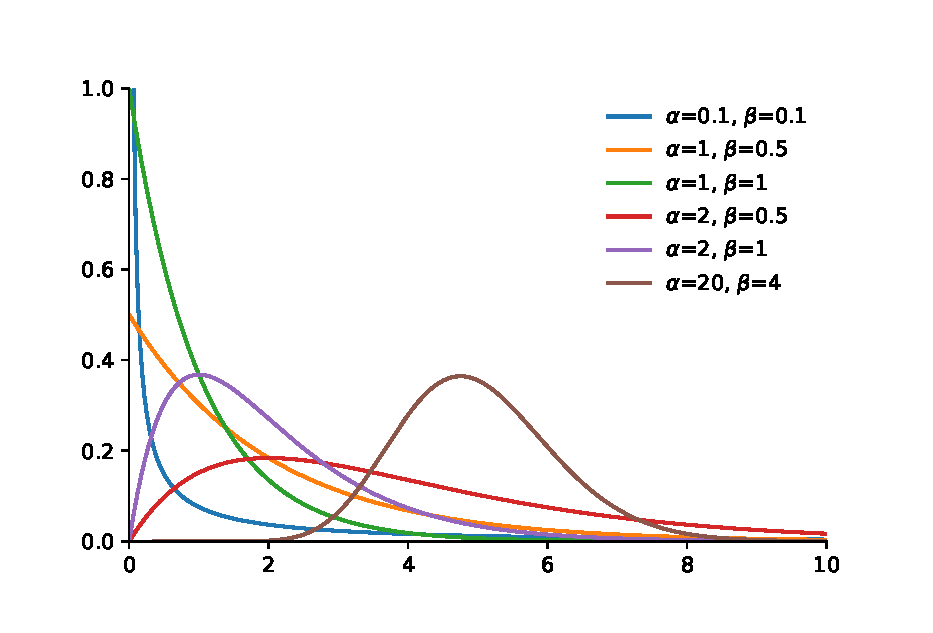
\includegraphics[width=0.8\textwidth]{ch3/gamma.eps}
    \caption{Función de densidad de probabilidad (pdf) de una distribución Gamma para diferentes parámetros de forma $\alpha$ y tasa $\beta$.}
    \label{img:gamma}
\end{figure}

\subsection{Configuración de hiperparámetros del grafo temporal}
\label{sec:graph_hiperparameters}

El grafo temporal cuenta con dos hiperparámetros: $q$ y $\zeta$. El parámetro $q \in [0,1]$ define el soporte de los tópicos, utilizando aquellas palabras más probables que explican q\% de la distribución acumulada del tópico. Por otro lado, el hiperparámetro $\zeta\in[0,1]$ define el úmbral de corte, representa el punto operante de la cdf del grafo \textit{fully-connected}, permite definir el cuantil que se usará como úmbral para eliminar arcos con similitud menor a este.\\

En cuanto al parámetro $q$ un valor razonable podría estar entre $[0.8, 0.95]$, de esta manera se conserva el \textit{core} de palabras del tópico y se disminuye de manera significativa el tiempo de cómputo. Por otro lado, valores razonables de $\zeta$ podrían estar entre $[0.9, 0.99]$, de esta manera solo se conservarían aquellas relaciones con una alta similitud relativa, debido a que el umbral de corte no depende de la medida de similitud utilizada.

\section{Resumen metodología}
\label{sec:methodology_resume}

En la Figura \ref{img:scheme} se presenta un esquema que resume la metodología propuesta para el descubrimiento y seguimiento de tópicos en el tiempo. En primer lugar, se divide el corpus original en épocas y a cada época se le aplican las siguientes cinco etapas en forma secuencial: tokenización, procesamiento de caracteres, eliminación de \textit{stopwords}, filtro por vocabulario y filtro por frecuencia. Como producto del proceso anterior se obtiene un corpus listo para la aplicación de un modelo de tópicos. En segundo lugar, se aplica HDP de forma independiente sobre cada una de las épocas. Por último, una vez descubiertos los tópicos se procede a construir el grafo temporal, para esto es necesario computar la WMD entre los tópicos de épocas adyacentes. Finalmente, se podan los arcos cuya similitud es menor al cuantil $\zeta$ de la distribución acumulada del grafo \textit{fully-connected}.

\def\db[#1,#2,#3,#4,#5]#6{%
  \node[draw, cylinder, alias=cyl, shape border rotate=90, aspect=#3, %
  minimum height=#1, minimum width=#2, outer sep=-0.5, color=black] (#4) at #5 {};%
  \node at #5 {#6};%
}
\def\boxtext[#1,#2,#3,#4,#5]#6{
        \node[draw=black, rounded corners, minimum height=#1,minimum width=#2, text width=6em] (#4) at #5 {}; 
        \node[anchor=#3,inner sep=4pt,] at (#4.#3)  {#6};
}
\def\isaedge[#1,#2,#3,#4];{ 
  \draw[-triangle 60,color=black!20!black,#4,fill=white] (#1) -- #3
  (#2);  
}

\begin{figure}
\begin{tikzpicture}
\db[45,40,1.6,db1,(0,2.2)] {
    \scriptsize\begin{tabular}{l}
        Corpus\\
        Original
    \end{tabular}
};
\boxtext[220,120,north,p,(3.5,2.2)] {\textbf{Procesamiento}};
\isaedge[db1,p,,];
\boxtext[180,100,south,p0,(3.5,2)] {$1:T$};
\boxtext[15,20,north,p1,(3.5,4.6)] {\footnotesize Tokenización};
\boxtext[15,20,north,p2,(3.5,3.4)]{\footnotesize Caracteres};
\boxtext[15,20,north,p3,(3.5,2.2)]{\footnotesize Stopwords};
\boxtext[15,20,north,p4,(3.5,1.0)]{\footnotesize Vocabulario};
\boxtext[15,20,north,p5,(3.5,-0.2)]{\footnotesize Frecuencia};
\isaedge[p1,p2,,];
\isaedge[p2,p3,,];
\isaedge[p3,p4,,];
\isaedge[p4,p5,,];
\db[45,40,1.6,db2,(7,2.2)] {
    \scriptsize\begin{tabular}{l}
        Corpus\\
        Procesado
    \end{tabular}
};
\isaedge[p,db2,,];
\boxtext[50,50,north,hdp,(9.7,2.2)] { 
    \begin{tabular}{l}
        \textbf{Tópicos}\\
        HDP $1:T$
    \end{tabular}
};
\isaedge[db2,hdp,,];
\boxtext[80,100,north,g,(13.5,2.2)] {\textbf{Grafo Temporal}};
\isaedge[hdp,g,,];
\boxtext[15,40,north,g1,(13.5,2.6)]{\footnotesize WMD};
\boxtext[15,40,north,g2,(13.5,1.4)]{\footnotesize Prunning};
\isaedge[g1,g2,,];
\end{tikzpicture}
\caption{Esquema de la metodología de descubrimiento y evolución de tópicos.}
\label{img:scheme}
\end{figure}


\chapter{Caso de estudio}
\label{ch:case_study}
En este capítulo se analizan los resultados de la metodología propuesta al fenómeno de robo de vehículos. En la sección \ref{sec:data} se describe la fuente de información utilizada. En la sección \ref{sec:data_processing} los resultados del procesamiento de los datos. Por último, en la sección \ref{sec:quantative}-\ref{sec:qualitative} se realiza un análisis cuantitativo y cualitativo de los resultados.

\section{Datos}
\label{sec:data}

Para este experimento se cuenta con relatos de víctimas del robo de vehículos provistos por la Asociación de Aseguradores de Chile (AACH). Esta base de datos consta con 49,015 relatos entre los años 2011-2016, veasé la Figura \ref{img:robberies_aach} para el detalle por año.

\begin{figure}
\includegraphics[width=0.8\textwidth]{ch4/robberies_aach.eps}
\caption{Cantidad de robos registrados por año en base de datos AACH.}
\label{img:robberies_aach}
\end{figure}

En la Figura \ref{img:documents} se muestra algunos ejemplos de la base de datos de la AACH, de aquí se observa que los relatos carecen de estandarización y presentan múltiples errores ortográficos. En consecuencia, la etapa de procesamiento toma suma relevancia, ya que aplicar un modelo de tópicos a un corpus sin ningún tipo de procesamiento puede llevar a resultados no deseados. En la sección \ref{sec:data_processing} se detallan los resultados obtenidos sobre el corpus tras aplicar los niveles de procesamiento mencionados en la sección \ref{sec:processing}.

\def\grayboxtext[#1,#2]#3{
        \node[fill=gray!80, text width=36em, draw=black!80, rounded corners, align=justify, below=#1] (#2) {#3}; 
}
\begin{figure}
\begin{tikzpicture}
    \grayboxtext[,t1]{\small ESTABA ESTACIONADO EL LA CALLE ROTEMBURGO ENTRE NORUGA Y SEÑORA DEL ROSAIO  Y AL MOMENTO DE IR A BUSCAR EL AUTO SE DA CUENTA QUE EL VH NO SE ENCUETRA AL PARECER LO ROBARON. NO POSEEE LOS DOCUMENTOS DEL VH vh aparece pero con mulples daños e evaluar queda en manos del liquidador.};
    \grayboxtext[0.2cm of t1,t2]{\small ME ENCONTRABA CARGANDO COMBUSTIBLE EN LA SHELL DE CARRASCAL CON WALKER MARTÍNEZ Y REPENTINAMENTE FUI ASALTADA EN FORMA VIOLENTA LLEVASE MI VEH (TENGO GRABACIÓN ). DAÑOS: ROBO DE MI VEH . LEIVA SE DERIVA A DON MARIO MEDINA .3 UF.DED/XX@XX.CL};
    \grayboxtext[0.2cm of t2,t3]{\small TEXT : DEJO MI VEHICULO ESTACIONADO EN DICHO LUGAR AL VOLVER ME PERCATO QUE EL VEHICULO HABIA SIDO ROBADO  EL MISMO DIA DEL ROBO A LAS 20:00 SOY CONTACTADO POR CARABINEROS DE LA COMUNA DE EL BOSQUE LOS CUALES ME INFORMAN QUE HABIAN RECUPERADO MI VEHICULO EL CUAL PRESENTABA LOS SIGUIENTES DAÑOS : VIDRIO TRASERO DERECHO QUEBRADA  CHAPA DE CONTACTO FORZADA  PARACHOQUE DELANTERO DERECHO RAYADO  ALARMADESCONECTADA  OTROS DAÑOS EN EL SISTEMA ELECTRICO  ALARMA DE AIRBAGS ENCENDIDA  ROBO DE ESPECIES.};
    \grayboxtext[0.2cm of t3,t4]{\small Descripción Siniestro: el dia 24 de abril se le arrendo el vh a XX el cual estuvo sin problemas pagando el arriendo  hasta el mes pasado que no pago mas y se le ha llamado en reiteradas veces y dice que va a venir a dejar el auto y no aparecel. por eso se realizo una denuncia por apropiacion indevida};
    \grayboxtext[0.2cm of t4,t5]{\small ammg  53966748    vh asegurado transitaba en calle copiapo alt. 750  en este punto sufro portonazo sujetos armados roban mi vh hoy a las 04.30am vh fue encontrado en sector de la pintana mi vh ahora esta siendo periciado.    daños por evaluar};
    \grayboxtext[0.2cm of t5,t6]{\small PATENTE XX Siendo las 22:30 en la interseccion de san Alfonso con Claudio Gay  un individuo me obliga a bajar del vehiculo apuntandome con una pistola  de inmediato aparecen dos personas mas  las que me suben en la parte trasera del furgon donde constantemente me amenazan con dispararme  me bajan del vehiculo en un potrero cercano a la autopista del sol  teniendome boca abajo golpeandome  luego me colocan un pa?o en la cara perdiendo el conocimiento  al despertar desorientado me dirijo a car};
\end{tikzpicture}
\caption{Muestra de relatos de la base de datos AACH.}
\label{img:documents}
\end{figure}

\section{Procesamiento}
\label{sec:data_processing}

En esta sección se detallan los resultados de aplicar el procesamiento descrito en la sección \ref{sec:processing}. Con fines gráficos los resultados del procesamiento se decriben en un orden distinto al descrito en dicha sección, con el objetivo de mostrar como estas afectan el tamaño del vocabulario. El orden es el siguiente, (i) tokenización, (ii) procesamiento de caracteres, (iii) eliminación de palabras poco frecuentes, (iv) filtro por vocabulario, (v) eliminación de \textit{stopwords} y (vi) eliminación de documentos con pocas palabras.\\

En primer lugar, se muestran la distribución acumulada del corpus original tras solo aplicar tokenización. Como se observa en la Figura \ref{img:cum_dist1} los \textit{tokens} totales corresponden a 2,030,980 asociado a un vocabulario de 93,203 palabras.\\

\begin{figure}
    \centering
    \includegraphics[trim={1.155cm 1.3cm 0 0},clip,width=0.6\textwidth]{ch4/cum_dist_1.eps}
    \caption{Frecuencia acumulada del vocabulario en orden decreciente de ocurrencia aplicando hasta el primer nivel de procesamiento.}
    \label{img:cum_dist1}
\end{figure}

En segundo lugar, se aplica la etapa de procesamiento de caracteres. De acuerdo a la Figura \ref{img:cum_dist2} el tamaño del vocabulario se reduce a casi la mitad, específicamente a 42,921 palabras, de forma similar la cantidad de \textit{tokens} se reduce a 1,028,412.

\begin{figure}
    \centering
    \includegraphics[trim={1.155cm 1.3cm 0 0},clip,width=0.6\textwidth]{ch4/cum_dist_2.eps}
    \caption{Frecuencia acumulada del vocabulario en orden decreciente de ocurrencia aplicando hasta el segundo nivel de procesamiento.}
    \label{img:cum_dist2}
\end{figure}

Hasta este nivel de procesamiento se tiene que cerca del 50\% de las palabras ocurren una única vez y al cerca de un 80\% tiene una frecuencia igual o menor a 4. El 95\% de la distribución acumulada puede ser explicada con 7,837 palabras (un 18\% del vocabulario actual). En conclusión, la distribución de las palabras tiene una cola bastante pesada.\\

En tercer lugar, se eliminan las palabras que aparecen en menos del 0.1\% de los documentos de su época. En la Figura \ref{img:cum_dist3} se muestra una reducción importante del vocabulario, específicamente a 3,148 (al rededor de 14 veces), reduciendo levemente  (alrededor de un 10\%) la cantidad de \textit{tokens} a 925,693.\\

\begin{figure}
    \centering
    \includegraphics[trim={1.155cm 1.3cm 0 0},clip,width=0.6\textwidth]{ch4/cum_dist_3.eps}
    \caption{Frecuencia acumulada del vocabulario en orden decreciente de ocurrencia aplicando hasta el tercer nivel de procesamiento.}
    \label{img:cum_dist3}
\end{figure}

En cuarto lugar, se filtran palabras usando el vocabulario extraído del SUC. En la Figura \ref{img:cum_dist4} se observa que el vocabulario se redujo a 2,902 y el la cantidad de \textit{tokens} a 901,745. En este caso la variación no fue menos significativa, alrededor de un 8\% en el tamaño del vocabulario y de un 3\% en el caso de los \textit{tokens}.\\

\begin{figure}
    \centering
    \includegraphics[trim={1.155cm 1.3cm 0 0},clip,width=0.6\textwidth]{ch4/cum_dist_4.eps}
    \caption{Frecuencia acumulada del vocabulario en orden decreciente de ocurrencia aplicando hasta el cuarto nivel de procesamiento.}
    \label{img:cum_dist4}
\end{figure}

En quinto lugar, se eliminan las \textit{stopwords}, de la Figura \ref{img:cum_dist5} se puede observar que significó una reducción significativa de tanto el vocabulario como del número de \textit{tokens}, respectivamente en 32\% (1,960 palabras) y 45\% (495,182 \textit{tokens}). La reducción abrupta en la cantidad de \textit{tokens} se debe principalmente a que las \textit{stopwords} son parte de las palabras más frecuentes dentro del corpus.\\

\begin{figure}
    \centering
    \includegraphics[trim={1.155cm 1.3cm 0 0},clip,width=0.6\textwidth]{ch4/cum_dist_5.eps}
    \caption{Frecuencia acumulada del vocabulario en orden decreciente de ocurrencia aplicando hasta el quinto nivel de procesamiento.}
    \label{img:cum_dist5}
\end{figure}

Por último, se eliminan los documentos con menos de 5 palabras, de la Figura \ref{img:cum_dist6} se puede observar que implicó una reducción de alrededor del 20\% en el tamaño del corpus y del 8\% en el número de \textit{tokens}.

\begin{figure}
    \centering
    \includegraphics[trim={1.155cm 1.3cm 0 0},clip,width=0.6\textwidth]{ch4/cum_dist_6.eps}
    \caption{Frecuencia acumulada del vocabulario en orden decreciente de ocurrencia aplicando hasta el sexto nivel de procesamiento.}
    \label{img:cum_dist6}
\end{figure}

En la tabla \ref{table:processing_stats} se muestra un cuadro resumen con estadísticas del corpus bajo distintos niveles de procesamiento. De aquí se extrae que el tamaño del vocabulario, el corpus y la cantidad de \textit{tokens} se redujo en alrededor de un 98\%, un 20\% y un 76\% respectivamente.

\begin{table}[H]
    \begin{tabular}{|c|c|c|c|}
    \hline
    procesamiento & documentos & vocabulario & tokens  \\ \hline
    t             & 49,015      & 93,203       & 2,030,980 \\ \hline
    t+ch          & 49,003      & 42,921       & 1,028,412 \\ \hline
    t+ch+f        & 48,988      & 3,148        & 925,693  \\ \hline
    t+ch+f+v      & 48,988      & 2,902        & 901,745  \\ \hline
    t+ch+f+v+s    & 48,566      & 1,960        & 495,182  \\ \hline
    t+ch+f+v+s+d  & 38,850      & 1,960        & 453,206  \\ \hline
    \end{tabular}
    \caption{Estadísticas del corpus bajo distintos niveles de procesamientos, \textbf{t}: tokenización, \textbf{ch}: procesamiento de caracteres, \textbf{f}: filtro por frecuencia, \textbf{v}: filtro por vocabulario, \textbf{s}: eliminación de \textit{stopwords}, \textbf{d}: eliminación de documentos.}
    \label{table:processing_stats}
    \end{table}

En la tabla \ref{table:innovation_rate} se muestra el detalle del vocabulario para cada una de las épocas tras procesar el corpus, de aquí se extrae que en promedio un 12.83\% del vocabulario se olvida de una época a otra y un 18.92\% es nuevo, en otras palabras, en promedio alrededor de un 32\% del vocabulario no es común entre tópicos de épocas adyacentes. Esto justifica la necesidad de utilizar medidas de similitud robustas a cambios en el vocabulario, permitiendo así una comparación más justa entre tópicos sin vocabulario común.

\begin{table}[H]
    \begin{tabular}{|c|r|r|r|r|}
    \hline
    \textbf{época} & \multicolumn{1}{c|}{\textbf{t-1}} & \multicolumn{1}{c|}{\textbf{t}} & \multicolumn{1}{c|}{\textbf{t-1 {[}\%{]}}} & \multicolumn{1}{l|}{\textbf{t {[}\%{]}}} \\ \hline
    2              & 1,145                              & 1,187                            & 14.41                                      & 18.08                                    \\ \hline
    3              & 1,187                              & 1,281                            & 13.56                                      & 21.48                                    \\ \hline
    4              & 1,281                              & 1,329                            & 13.35                                      & 17.10                                    \\ \hline
    5              & 1,329                              & 1,405                            & 12.57                                      & 18.28                                    \\ \hline
    6              & 1,405                              & 1,537                            & 10.25                                      & 19.64                                    \\ \hline
    \end{tabular}
    \caption{Evolución del vocabulario en el tiempo, \textbf{t-1}: corresponde al vocabulario del período anterior a la época respectiva, \textbf{t}: corresponde al vocabulario de la época actual, \textbf{t-1[\%]}: porcentaje de palabras del período $t-1$ que ya no están en el período $t$ y \textbf{t[\%]}: porcentaje de palabras del período $t$ que no están en el período $t-1$.}
    \label{table:innovation_rate}.
\end{table}


\section{Análisis cuantitativo de resultados}
\label{sec:quantative}

En esta sección se describen los resultados cuantitativos de aplicar la metodología propuesta al corpus descrito en la sección \ref{sec:data}. En primer lugar, se analiza el comportamiento temporal de los tópicos bajo distintos puntos operantes $\zeta$ para podar el grafo \textit{fully-connected}. En segundo lugar, se analizan los resultados de aplicar la heurística descrita en \ref{sec:wmd_complexity}, la cual mejora los tiempos de construcción del grafo de similitud a costa de pérdida en precisión.

\subsection{Grafo de similitud temporal}

Como se menciona en la sección \ref{sec:build_graph}, el grafo temporal se construye relacionando los tópicos de épocas adyacentes a través de una medida de similitud, los tópicos son descubiertos usando el modelo HDP y WMD por medida de similitud. En base a un punto operante $\zeta \in [0,1]$ de la cdf de la similitud del grafo completo se determina el úmbral de corte. Aquellos arcos con similitud menor a este úmbral son eliminados. De esta forma la elección del úmbral no depende fuertemente de la medida de similitud escogida. En la Figura \ref{img:cdf_wmd} se ilustra la cdf del grafo \textit{fully-connected} obtenido de aplicar la metodología propuesta al corpus descrito en la sección \ref{sec:data}.

\begin{figure}
    \centering
    \includegraphics[width=\textwidth]{ch4/cdf.eps}
    \caption{Estimación empírica de la cdf de la similitud WMD entre tópicos del grafo \textit{fully-conected}.}
    \label{img:cdf_wmd}
\end{figure}

En la Figura \ref{img:temporal_similarity_graphs} se muestran los grafos resultantes tras aplicar distintos puntos operantes $\zeta$. Como es esperado, un incremento de $\zeta$ resulta en un incremento en la \textit{sparsity} del grafo temporal.

\begin{figure}
\centering
\subfloat[$\zeta$ = 0]{
  \includegraphics[width=0.4\textwidth]{ch4/graph_q100.png}
}
\subfloat[$\zeta$ = 0.9]{
  \includegraphics[width=0.4\textwidth]{ch4/graph_q100_e90.png}
}\\
\subfloat[$\zeta$ = 0.95]{
  \includegraphics[width=0.4\textwidth]{ch4/graph_q100_e95.png}
}
\subfloat[$\zeta$ = 0.99]{
  \includegraphics[width=0.4\textwidth]{ch4/graph_q100_e99.png}
}\\
\caption{Grafo de similitud temporal. Los tres grafos corresponden al mismo corpus y fueron construidos usando el mismo conjunto de tópicos con WMD como medida de similitud, pero bajo diferentes puntos operantes $\zeta$ de la CDF. El eje horizontal denota el tiempo en años, partiendo en el 2011 hasta el 2016, donde cada columna de tópicos corresponde a una época específica. Mientras más claro sea el color del nodo que representa un tópico más popularidad posee en su correspondiente época y mientras mayor es el grosor del arco entre dos tópicos mayor es su similitud.}
\label{img:temporal_similarity_graphs}
\end{figure}


En el grafo podado se pueden identificar diferentes dinamismos en cada época, como nacimiente, muerte, evolución, fusión y división. Un tópico nace en una época si en la época anterior no posee antecesores. La época de muerte de un tópico se identifica como aquella en que no tiene ningún descendiente. Un tópico evoluciona si posee un único antecesor. La fusión ocurre en una época cuando un tópico tiene más de un antecesor. En cambio, la división ocurre cuando hay dos o más tópicos de una época que comparten un antecesor.\\

En la Figura \ref{img:topics_evolution} se muestra la proporción de tópicos que nacen, mueren, fusionan, y dividen por época, normalizando por el número total de tópicos inferido en esa época. Se puede observar que al incrementar $\zeta$ la proporción de tópicos que nacen y mueren aumenta significativamente, puesto que al ser mayor el úmbral de corte menos ascendentes y descendientes se tienen, por otro lado, la división y fusión decrecen, debido a la menor presencia de conexiones.

\begin{figure}
    \centering
    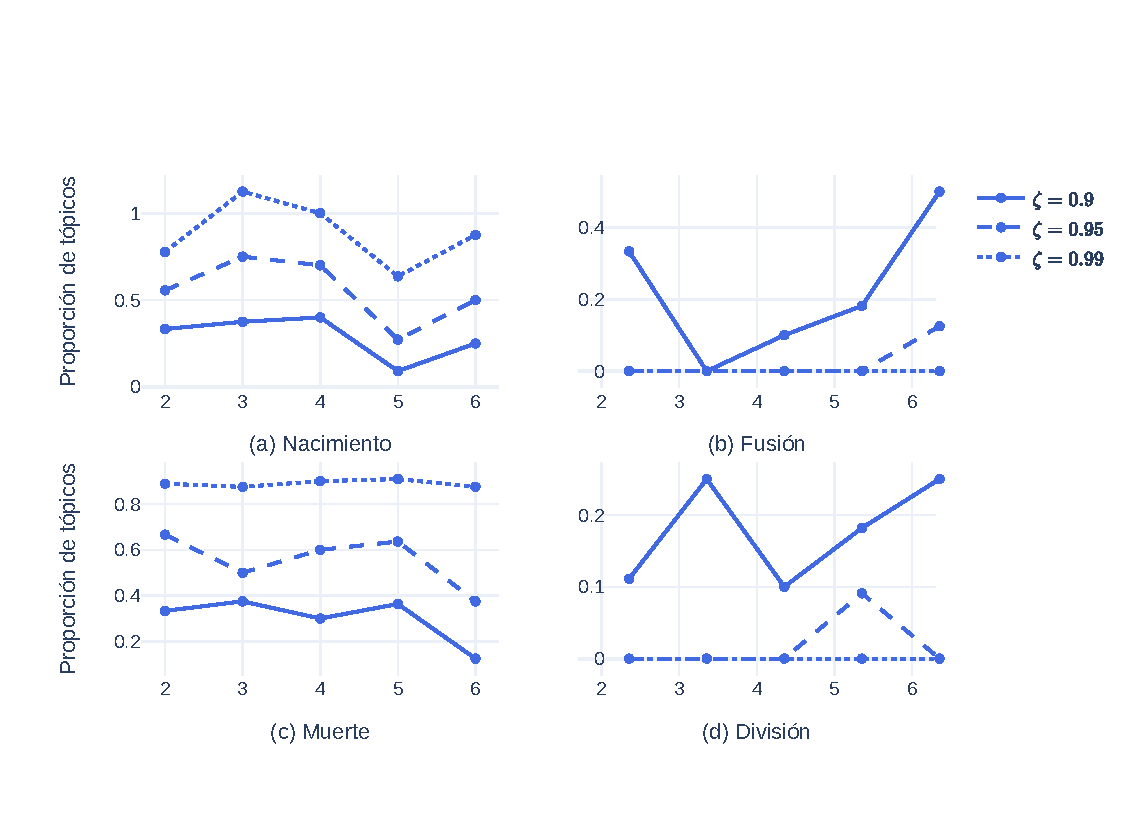
\includegraphics[width=\textwidth]{ch4/topics_evolution.eps}
    \caption{Proporción de tópicos que nacen, mueren, fusionan y dividen por época, normalizando por el número total de tópicos inferido en esa época, bajo diferentes puntos operantes $\zeta$.}
    \label{img:topics_evolution}
\end{figure}



\subsection{Heurística de mejora del tiempo de construcción del grafo de similitud}

WMD es una medida intensiva en recursos computacionales, por lo que se requiere de heurísticas para escalar la metodología a un gran volumen de datos. Como se menciona en la sección \ref{sec:wmd_complexity} una forma de reducir significativamente el tiempo de creación del grafo temporal es utilzar el top N de palabras más probables del tópico que expliquen determinado porcentaje de la distribución acumulada. A la hora de aplicar esta heurística se debe tener en cuenta la posible pérdida de información al representar un tópico con un vocabulario reducido. Sea $G_{\zeta}$ el grafo obtenido al aplicar tras podar el grafo completo con un punto operante $\zeta$ y $G^{'}_{\zeta}$ el grafo aproximado de aplicar la heurística, con $E$ y $E^{'}$ los conjuntos de arcos respectivos. Luego, el porcentaje de arcos correctos de la heurística corresponde a la cardinalidad de la intersección divida por la cardinalidad de la unión, matemáticamente:

\begin{equation}
  \frac{|E\cap E^{'}|}{|E\cup E^{'}|}
\end{equation}

En la Figura \ref{img:speedup} se muestra la mejora en \textit{speedup} y el incremento en error al usar un porcentaje menor de la cdf del tópico para construir el grafo de similitud temporal. Utilizando el 20\% de la cdf la construcción del grafo de similitud disminuye en más de 1,207 veces, esto bajo un error medianamente aceptable del orden del 10-30\%. Si se utiliza un 60\% de la cdf el tiempo mejora en casi 137 veces, siendo el error menor al 10\%. Por otro lado, si se utiliza un 90\% de la cdf el error es inferior al 5\%, siendo el speedup es aproximadamente 8 veces superior a utilizar el vocabulario completo del tópico en la construcción del grafo temporal.

\begin{figure}
    \centering
    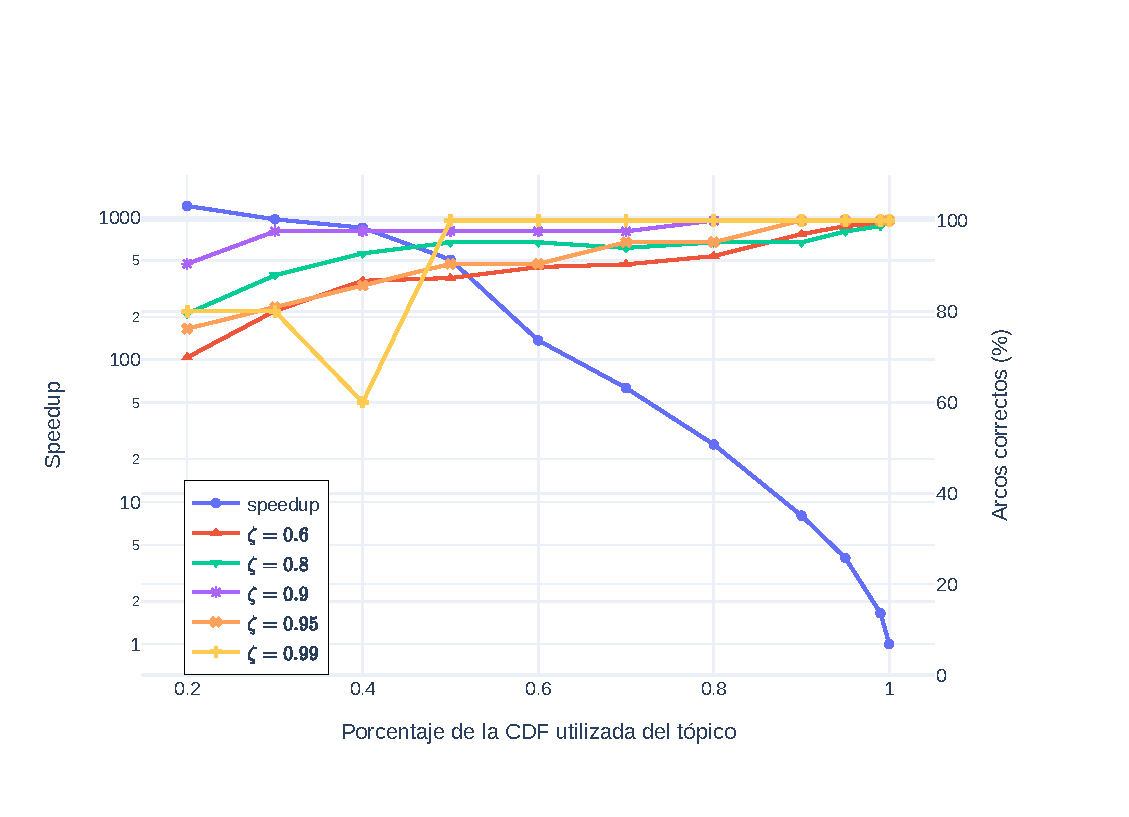
\includegraphics[width=\textwidth]{ch4/speedup.eps}
    \caption{\textit{Speedup} y porcentaje de arcos correctos al utilizar un menor porcentaje de la cdf de los tópicos en la construcción del grafo de similitud. El error de la heurística es mostrado para diferentes puntos operantes $\zeta$ utilizados para podar el grafo completo.} 
    \label{img:speedup}
\end{figure}


\section{Análisis cualitativo de resultados}
\label{sec:qualitative}

En esta sección se realiza un análisis cualitativo de los tópicos descubiertos y su evolución. El análisis es realizado sobre el grafo podado con un punto operante $\zeta = 0.95$ mostrado en la Figura \ref{img:temporal_similarity_graphs}. En las siguientes dos subsecciones se analizan los dos tópicos más predominantes en el tiempo: en la sección \ref{sec:noviolence_topic} se estudia el robo no presencial y en la sección \ref{sec:violence_topic} se analiza el robo con violencia.

\subsection{Evolución del robo no presencial}
\label{sec:noviolence_topic}

En la Figura \ref{img:noviolence_topic} se muestra la evolución de uno de los tópicos más predominantes del grafo temporal. A diferencia de otros tópicos este tópico no presenta en el tiempo división, fusión ni desaparición. En base a las top 10 palabras más probables el tópico se puede caracterizar como un robo bajo las siguientes circunstancias: vehículo estacionado en la calle, sin la presencia del conductor, el conductor al regresar al lugar se percata de la ausencia del vehículo. Un nombre adecuado para este tópico podría ser \quotes{robo no presencial}, ya que se caracteriza por no contar con la presencia del conductor cuando ocurre el robo. Este tópico se caracteriza por su gran estabilidad en el tiempo, ya que en el top 10 se encuentran practicamente las mismas palabras. Por último, se observa una tendencia a la baja de la participación del tópico, en el año 2011 alrededor del 44\% de los \textit{tokens} provienen de este tópico y en el año 2016 se tiene un 32\%.


\def\topic[#1,#2,#3,#4,#5,#6]#7{
        \node[fill=#1, rounded corners, minimum height=#2, minimum width=#3, text width=4em] (#5) at #6 {}; 
        \node[anchor=#4,inner sep=2pt,] at (#5.#4)  {#7};
}
\def\tedge[#1,#2,#3,#4,#5];{ 
  \definecolor{color0}{RGB}{153,153,153}
  \draw[color=color0,#4,fill=white, line width=4*#5pt] (#1) -- #3
  (#2);  
}

\definecolor{color1}{RGB}{184,222,41}
\definecolor{color2}{RGB}{253,231,37}
\definecolor{color3}{RGB}{134,213,73}
\definecolor{color4}{RGB}{127,211,78}
\definecolor{color5}{RGB}{52,182,121}
\definecolor{color6}{RGB}{40,174,128}

\begin{figure}
\begin{tikzpicture}
  \topic[color1,60,80,north,t1,(0,0)] {
     \scriptsize
     \begin{tabular}{l}
       estacionado deje\\
       calle encontraba\\
       lugar regresar\\
       domicilio volver\\
       percato salir
     \end{tabular}
  }
  \topic[color2,60,80,north,t2,(3,0)] {
     \scriptsize
     \begin{tabular}{l}
       estacionado deje\\
       calle lugar\\
       encontraba domicilio\\
       percato salir\\
       volver regresar
     \end{tabular}
  };
  \topic[color3,60,80,north,t3,(6,0)] {
     \scriptsize
     \begin{tabular}{l}
       estacionado deje\\
       calle encontraba\\
       lugar percato\\
       domicilio frente\\
       regresar salir
     \end{tabular}
  };
  \topic[color4,60,80,north,t4,(9,0)] {
     \scriptsize
     \begin{tabular}{l}
       estacionado deje\\
       calle lugar\\
       encontraba domicilio\\
       percato volver\\
       dejo salir
     \end{tabular}
  };
  \topic[color5,60,80,north,t5,(12,0)] {
     \scriptsize
     \begin{tabular}{l}
       estacionado deje\\
       calle lugar\\
       encontraba percato\\
       domicilio volver\\
       salir dejo
     \end{tabular}
  };
  \topic[color6,60,80,north,t6,(15,0)] {
     \scriptsize
     \begin{tabular}{l}
       estacionado deje\\
       calle lugar\\
       econtraba percato\\
       salir camioneta\\
       dejo domicilio
     \end{tabular}
  };
  \tedge[t1,t2,,,0.625];
  \tedge[t2,t3,,,0.586];
  \tedge[t3,t4,,,0.581];
  \tedge[t4,t5,,,0.632];
  \tedge[t5,t6,,,0.609];
\end{tikzpicture}
\caption{Evolución del tópico de robo de vehículo no presecial. El eje horizontal denota el tiempo en años, partiendo en el 2011 hasta el 2016. Mientras más claro el color del tópico más popularidad posee en su correspondiente época y mientras mayor es el grosor del arco entre dos tópicos mayor es su similitud.}
\label{img:noviolence_topic}
\end{figure}

\subsection{Evolución del robo con violenca}
\label{sec:violence_topic}

En la Figura \ref{img:violence_topic} se describe un tipo de robo de vehículo que se puede clasificar como robo con violencia. Este delito, se presenta de la siguiente forma: un conjunto de personas se bajan de un vehículo, intimidan al conductor mediante una pistola u otra arma de fuego, le quitan las llaves del vehículo y finalmente se llevan el vehículo dándose a la fuga. La participación de este tipo de robo se ha visto al alza, en el 2011 su participación era del 12\% y en el 2016 del 36\%, por lo que se ha convertido en un delito más a la moda, quitandole terreno al robo no presencial. A diferencia del tópico robo no presencial este presenta una fusión y división en el 2015. En ese año emerge del robo con violencia un subtópico popularmente conocido como \quotes{portonazo}, un robo con violencia que se caracteriza por la sustracción del vehículo en el portón de la casa de la víctima. Ese año coincide con la popularización de aquel \textit{modus operandi}. Al siguiente año el subtópico se vuelve a fusionar para formar parte del tópico robo con violencia de períodos anteriores.

\definecolor{color1}{RGB}{50,100,142}
\definecolor{color2}{RGB}{48,105,142}
\definecolor{color3}{RGB}{43,116,142}
\definecolor{color4}{RGB}{44,115,142}
\definecolor{color51}{RGB}{37,133,142}
\definecolor{color52}{RGB}{48,106,142}
\definecolor{color6}{RGB}{78,195,107}

\begin{figure}
\begin{tikzpicture}
  \topic[color1,60,80,north,t1,(0,0)] {
     \scriptsize
     \begin{tabular}{l}
       arma personas\\
       tipos individuos\\
       llaves fuego\\
       calle pistola\\
       llevaron bajar
     \end{tabular}
  }
  \topic[color2,60,80,north,t2,(3,0)] {
     \scriptsize
     \begin{tabular}{l}
       llaves personas\\
       individuos tipos\\
       calle persona\\
       arma pistola\\
       bajar llevaron
     \end{tabular}
  };
  \topic[color3,60,80,north,t3,(6,0)] {
     \scriptsize
     \begin{tabular}{l}
       personas calle\\
       llaves individuos\\
       arma pistola\\
       fuego tipos\\
       llevaron fuga
     \end{tabular}
  };
  \topic[color4,60,80,north,t4,(9,0)] {
     \scriptsize
     \begin{tabular}{l}
       personas individuos\\
       tipos calle\\
       llaves arma\\
       llevaron sujetos\\
       fuego armas
     \end{tabular}
  };
  \topic[color51,60,80,north,t51,(12,1.2)] {
     \scriptsize
     \begin{tabular}{l}
       bajan individuos\\
       llaves armas\\
       algun calle\\
       fuego personas\\
       sujetos todas
     \end{tabular}
  };
  \topic[color52,60,80,north,t52,(12,-1.2)] {
     \scriptsize
     \begin{tabular}{l}
       llavas tipos\\
       pitola personas\\
       casa llevaron\\
       bajaron arma\\
       porton puerta
     \end{tabular}
  };
  \topic[color6,60,80,north,t6,(15,0)] {
     \scriptsize
     \begin{tabular}{l}
       estacionado deje\\
       calle lugar\\
       econtraba percato\\
       salir camioneta\\
       dejo domicilio
     \end{tabular}
  };
  \tedge[t1,t2,,,0.499];
  \tedge[t2,t3,,,0.498];
  \tedge[t3,t4,,,0.5];
  \tedge[t4,t51,,,0.422];
  \tedge[t4,t52,,,0.405];
  \tedge[t51,t6,,,0.395];
  \tedge[t52,t6,,,0.483];
\end{tikzpicture}
\caption{Evolución del tópico de robo con violencia de vehículo. El eje horizontal denota el tiempo en años, partiendo en el 2011 hasta el 2016. Mientras más claro el color del tópico más popularidad posee en su correspondiente época y mientras mayor es el grosor del arco entre dos tópicos mayor es su similitud.}
\label{img:violence_topic}
\end{figure}


\chapter{Conclusiones y trabajo futuro}
\label{ch:conclusion}
\todosec[inline]{Conclusiones}

\todosec[inline]{Otras aplicaciones}

\todosec[inline]{Trabajo futuro}

\bibliography{main}

% FIN DEL DOCUMENTO
\end{document}